\documentclass[12pt,]{book}
\usepackage{lmodern}
\usepackage{amssymb,amsmath}
\usepackage{ifxetex,ifluatex}
\usepackage{fixltx2e} % provides \textsubscript
\ifnum 0\ifxetex 1\fi\ifluatex 1\fi=0 % if pdftex
  \usepackage[T1]{fontenc}
  \usepackage[utf8]{inputenc}
\else % if luatex or xelatex
  \ifxetex
    \usepackage{mathspec}
  \else
    \usepackage{fontspec}
  \fi
  \defaultfontfeatures{Ligatures=TeX,Scale=MatchLowercase}
\fi
% use upquote if available, for straight quotes in verbatim environments
\IfFileExists{upquote.sty}{\usepackage{upquote}}{}
% use microtype if available
\IfFileExists{microtype.sty}{%
\usepackage{microtype}
\UseMicrotypeSet[protrusion]{basicmath} % disable protrusion for tt fonts
}{}
\usepackage[left=2.54cm, right=2.54cm, top=2.54cm, bottom=2.54cm]{geometry}
\usepackage{hyperref}
\PassOptionsToPackage{usenames,dvipsnames}{color} % color is loaded by hyperref
\hypersetup{unicode=true,
            pdftitle={PRIORITIZR WORKSHOP MANUAL},
            pdfauthor={Jeffrey O. Hanson},
            colorlinks=true,
            linkcolor=Maroon,
            citecolor=Blue,
            urlcolor=blue,
            breaklinks=true}
\urlstyle{same}  % don't use monospace font for urls
\usepackage{natbib}
\bibliographystyle{plainnat}
\usepackage{color}
\usepackage{fancyvrb}
\newcommand{\VerbBar}{|}
\newcommand{\VERB}{\Verb[commandchars=\\\{\}]}
\DefineVerbatimEnvironment{Highlighting}{Verbatim}{commandchars=\\\{\}}
% Add ',fontsize=\small' for more characters per line
\usepackage{framed}
\definecolor{shadecolor}{RGB}{248,248,248}
\newenvironment{Shaded}{\begin{snugshade}}{\end{snugshade}}
\newcommand{\KeywordTok}[1]{\textcolor[rgb]{0.13,0.29,0.53}{\textbf{#1}}}
\newcommand{\DataTypeTok}[1]{\textcolor[rgb]{0.13,0.29,0.53}{#1}}
\newcommand{\DecValTok}[1]{\textcolor[rgb]{0.00,0.00,0.81}{#1}}
\newcommand{\BaseNTok}[1]{\textcolor[rgb]{0.00,0.00,0.81}{#1}}
\newcommand{\FloatTok}[1]{\textcolor[rgb]{0.00,0.00,0.81}{#1}}
\newcommand{\ConstantTok}[1]{\textcolor[rgb]{0.00,0.00,0.00}{#1}}
\newcommand{\CharTok}[1]{\textcolor[rgb]{0.31,0.60,0.02}{#1}}
\newcommand{\SpecialCharTok}[1]{\textcolor[rgb]{0.00,0.00,0.00}{#1}}
\newcommand{\StringTok}[1]{\textcolor[rgb]{0.31,0.60,0.02}{#1}}
\newcommand{\VerbatimStringTok}[1]{\textcolor[rgb]{0.31,0.60,0.02}{#1}}
\newcommand{\SpecialStringTok}[1]{\textcolor[rgb]{0.31,0.60,0.02}{#1}}
\newcommand{\ImportTok}[1]{#1}
\newcommand{\CommentTok}[1]{\textcolor[rgb]{0.56,0.35,0.01}{\textit{#1}}}
\newcommand{\DocumentationTok}[1]{\textcolor[rgb]{0.56,0.35,0.01}{\textbf{\textit{#1}}}}
\newcommand{\AnnotationTok}[1]{\textcolor[rgb]{0.56,0.35,0.01}{\textbf{\textit{#1}}}}
\newcommand{\CommentVarTok}[1]{\textcolor[rgb]{0.56,0.35,0.01}{\textbf{\textit{#1}}}}
\newcommand{\OtherTok}[1]{\textcolor[rgb]{0.56,0.35,0.01}{#1}}
\newcommand{\FunctionTok}[1]{\textcolor[rgb]{0.00,0.00,0.00}{#1}}
\newcommand{\VariableTok}[1]{\textcolor[rgb]{0.00,0.00,0.00}{#1}}
\newcommand{\ControlFlowTok}[1]{\textcolor[rgb]{0.13,0.29,0.53}{\textbf{#1}}}
\newcommand{\OperatorTok}[1]{\textcolor[rgb]{0.81,0.36,0.00}{\textbf{#1}}}
\newcommand{\BuiltInTok}[1]{#1}
\newcommand{\ExtensionTok}[1]{#1}
\newcommand{\PreprocessorTok}[1]{\textcolor[rgb]{0.56,0.35,0.01}{\textit{#1}}}
\newcommand{\AttributeTok}[1]{\textcolor[rgb]{0.77,0.63,0.00}{#1}}
\newcommand{\RegionMarkerTok}[1]{#1}
\newcommand{\InformationTok}[1]{\textcolor[rgb]{0.56,0.35,0.01}{\textbf{\textit{#1}}}}
\newcommand{\WarningTok}[1]{\textcolor[rgb]{0.56,0.35,0.01}{\textbf{\textit{#1}}}}
\newcommand{\AlertTok}[1]{\textcolor[rgb]{0.94,0.16,0.16}{#1}}
\newcommand{\ErrorTok}[1]{\textcolor[rgb]{0.64,0.00,0.00}{\textbf{#1}}}
\newcommand{\NormalTok}[1]{#1}
\usepackage{longtable,booktabs}
\usepackage{graphicx,grffile}
\makeatletter
\def\maxwidth{\ifdim\Gin@nat@width>\linewidth\linewidth\else\Gin@nat@width\fi}
\def\maxheight{\ifdim\Gin@nat@height>\textheight\textheight\else\Gin@nat@height\fi}
\makeatother
% Scale images if necessary, so that they will not overflow the page
% margins by default, and it is still possible to overwrite the defaults
% using explicit options in \includegraphics[width, height, ...]{}
\setkeys{Gin}{width=\maxwidth,height=\maxheight,keepaspectratio}
\IfFileExists{parskip.sty}{%
\usepackage{parskip}
}{% else
\setlength{\parindent}{0pt}
\setlength{\parskip}{6pt plus 2pt minus 1pt}
}
\setlength{\emergencystretch}{3em}  % prevent overfull lines
\providecommand{\tightlist}{%
  \setlength{\itemsep}{0pt}\setlength{\parskip}{0pt}}
\setcounter{secnumdepth}{5}
% Redefines (sub)paragraphs to behave more like sections
\ifx\paragraph\undefined\else
\let\oldparagraph\paragraph
\renewcommand{\paragraph}[1]{\oldparagraph{#1}\mbox{}}
\fi
\ifx\subparagraph\undefined\else
\let\oldsubparagraph\subparagraph
\renewcommand{\subparagraph}[1]{\oldsubparagraph{#1}\mbox{}}
\fi

%%% Use protect on footnotes to avoid problems with footnotes in titles
\let\rmarkdownfootnote\footnote%
\def\footnote{\protect\rmarkdownfootnote}

%%% Change title format to be more compact
\usepackage{titling}

% Create subtitle command for use in maketitle
\providecommand{\subtitle}[1]{
  \posttitle{
    \begin{center}\large#1\end{center}
    }
}

\setlength{\droptitle}{-2em}

  \title{PRIORITIZR WORKSHOP MANUAL}
    \pretitle{\vspace{\droptitle}\centering\huge}
  \posttitle{\par}
    \author{Jeffrey O. Hanson}
    \preauthor{\centering\large\emph}
  \postauthor{\par}
      \predate{\centering\large\emph}
  \postdate{\par}
    \date{2019-10-06}

% load packages
\usepackage{caption}
\usepackage{float}

% default bookdown preamble
\usepackage{booktabs}
\usepackage{amsthm}
\makeatletter
\def\thm@space@setup{%
  \thm@preskip=8pt plus 2pt minus 4pt
  \thm@postskip=\thm@preskip
}
\makeatother

% remove figure labelling
\captionsetup[figure]{labelformat=empty,textfont=it}

% make figures static
\let\origfigure\figure
\let\endorigfigure\endfigure
\renewenvironment{figure}[1][2] {
  \expandafter\origfigure\expandafter[H]
} {
  \endorigfigure
}

% text boxes
\ifxetex
  \usepackage{letltxmacro}
  \setlength{\XeTeXLinkMargin}{1pt}
  \LetLtxMacro\SavedIncludeGraphics\includegraphics
  \def\includegraphics#1#{% #1 catches optional stuff (star/opt. arg.)
    \IncludeGraphicsAux{#1}%
  }%
  \newcommand*{\IncludeGraphicsAux}[2]{%
    \XeTeXLinkBox{%
      \SavedIncludeGraphics#1{#2}%
    }%
  }%
\fi

\makeatletter
\newenvironment{kframe}{%
\medskip{}
\setlength{\fboxsep}{.8em}
 \def\at@end@of@kframe{}%
 \ifinner\ifhmode%
  \def\at@end@of@kframe{\end{minipage}}%
  \begin{minipage}{\columnwidth}%
 \fi\fi%
 \def\FrameCommand##1{\hskip\@totalleftmargin \hskip-\fboxsep
 \colorbox{shadecolor}{##1}\hskip-\fboxsep
     % There is no \\@totalrightmargin, so:
     \hskip-\linewidth \hskip-\@totalleftmargin \hskip\columnwidth}%
 \MakeFramed {\advance\hsize-\width
   \@totalleftmargin\z@ \linewidth\hsize
   \@setminipage}}%
 {\par\unskip\endMakeFramed%
 \at@end@of@kframe}
\makeatother

\makeatletter
\@ifundefined{Shaded}{
}{\renewenvironment{Shaded}{\begin{kframe}}{\end{kframe}}}
\makeatother

\newenvironment{rmdblock}[1]
  {
  \begin{itemize}
  \renewcommand{\labelitemi}{
    \raisebox{-.7\height}[0pt][0pt]{
      {\setkeys{Gin}{width=3em,keepaspectratio}\includegraphics{images/#1}}
    }
  }
  \setlength{\fboxsep}{1em}
  \begin{kframe}
  \item
  }
  {
  \end{kframe}
  \end{itemize}
  }
\newenvironment{rmdnote}
  {\begin{rmdblock}{note}}
  {\end{rmdblock}}
\newenvironment{rmdcaution}
  {\begin{rmdblock}{caution}}
  {\end{rmdblock}}
\newenvironment{rmdquestion}
  {\begin{rmdblock}{question}}
  {\end{rmdblock}}
\newenvironment{rmdanswer}
  {\begin{rmdblock}{answer}}
  {\end{rmdblock}}
\newenvironment{rmdimportant}
  {\begin{rmdblock}{important}}
  {\end{rmdblock}}
\newenvironment{rmdtip}
  {\begin{rmdblock}{tip}}
  {\end{rmdblock}}
\newenvironment{rmdwarning}
  {\begin{rmdblock}{warning}}
  {\end{rmdblock}}

\let\BeginKnitrBlock\begin \let\EndKnitrBlock\end
\begin{document}
\maketitle

{
\hypersetup{linkcolor=black}
\setcounter{tocdepth}{0}
\tableofcontents
}
\chapter{Welcome!}\label{welcome}

Here you will find the manual for the prioritizr module of the
\href{https://cibio.up.pt/workshops--courses/details/advanced-course-spatial-conservation-prioritization-}{\emph{Spatial
Conservation Prioritization: Concepts, Methods and Application}
workshop} held at CIBIO-InBIO, Vairão, Portugal. \textbf{Before you
arrive at the workshop, you should make sure that you have correctly
\protect\hyperlink{setup}{set up your computer for the workshop} and you
have
\href{https://github.com/prioritizr/cibio-workshop/raw/master/data.zip}{downloaded
the data from here}. We cannot guarantee a reliable Internet connection
during the workshop, and so you may be unable to complete the workshop
if you have not set up your computer beforehand.}

\chapter{Introduction}\label{introduction}

\section{Overview}\label{overview}

The aim of this workshop is to help you get started with using the
prioritizr R package for systematic conservation planning. It is not
designed to give you a comprehensive overview and you will not become an
expert after completing this workshop. Instead, we want to help you
understand the core principles of conservation planning and guide you
through some of the common tasks involved with developing
prioritizations. In other words, we want to give you the knowledge base
and confidence needed to start applying systematic conservation planning
to your own work.

You are not alone in this workshop. If you are having trouble, please
put your hand up and one of the instructors will help you as soon as
they can. You can also ask the people sitting next to you for help too.
\textbf{Most importantly, the code needed to answer the questions in
this workshop are almost always located in the same section as the
question. So if you are stuck, try rereading the example code and see if
you can modify it to answer the question.} Please note that the first
thing an instructor will ask you will (probably) be ``what have you
tried so far?''. We can't help you if you haven't tried anything.

\hypertarget{setup}{\section{Setting up your computer}\label{setup}}

You will need to have both \href{https://www.r-project.org}{R} and
\href{https://www.rstudio.com/}{RStudio} installed on your computer to
complete this workshop. Although it is not imperative that you have the
latest version of RStudio installed, \textbf{you will need the latest
version of R installed (i.e.~version 3.6.1)}. Please note that you meed
need administrative permissions to complete install these programs.
After installing them, you will also need to install various R packages
too.

\subsection{R}\label{r}

The \href{https://www.r-project.org}{R statistical computing
environment} can be downloaded from the Comprehensive R Archive Network
(CRAN). You can download the latest version of R (version 3.6.1) from
here: \url{https://cloud.r-project.org}. Please note that you will need
to download the correct file for your operating system (i.e.~Linux, Mac
OSX, Windows).

\subsection{RStudio}\label{rstudio}

\href{https://www.rstudio.com}{RStudio} is an integrated development
environment (IDE). In other words, it is a program that is designed to
make your R programming experience more enjoyable. During this workshop,
you will interact with R through RStudio---meaning that you will open
RStudio when you want to code in R. You can download the latest version
of RStudio here: \url{http://www.rstudio.com/download}. When you start
RStudio, you will see two main parts of the interface:

\begin{center}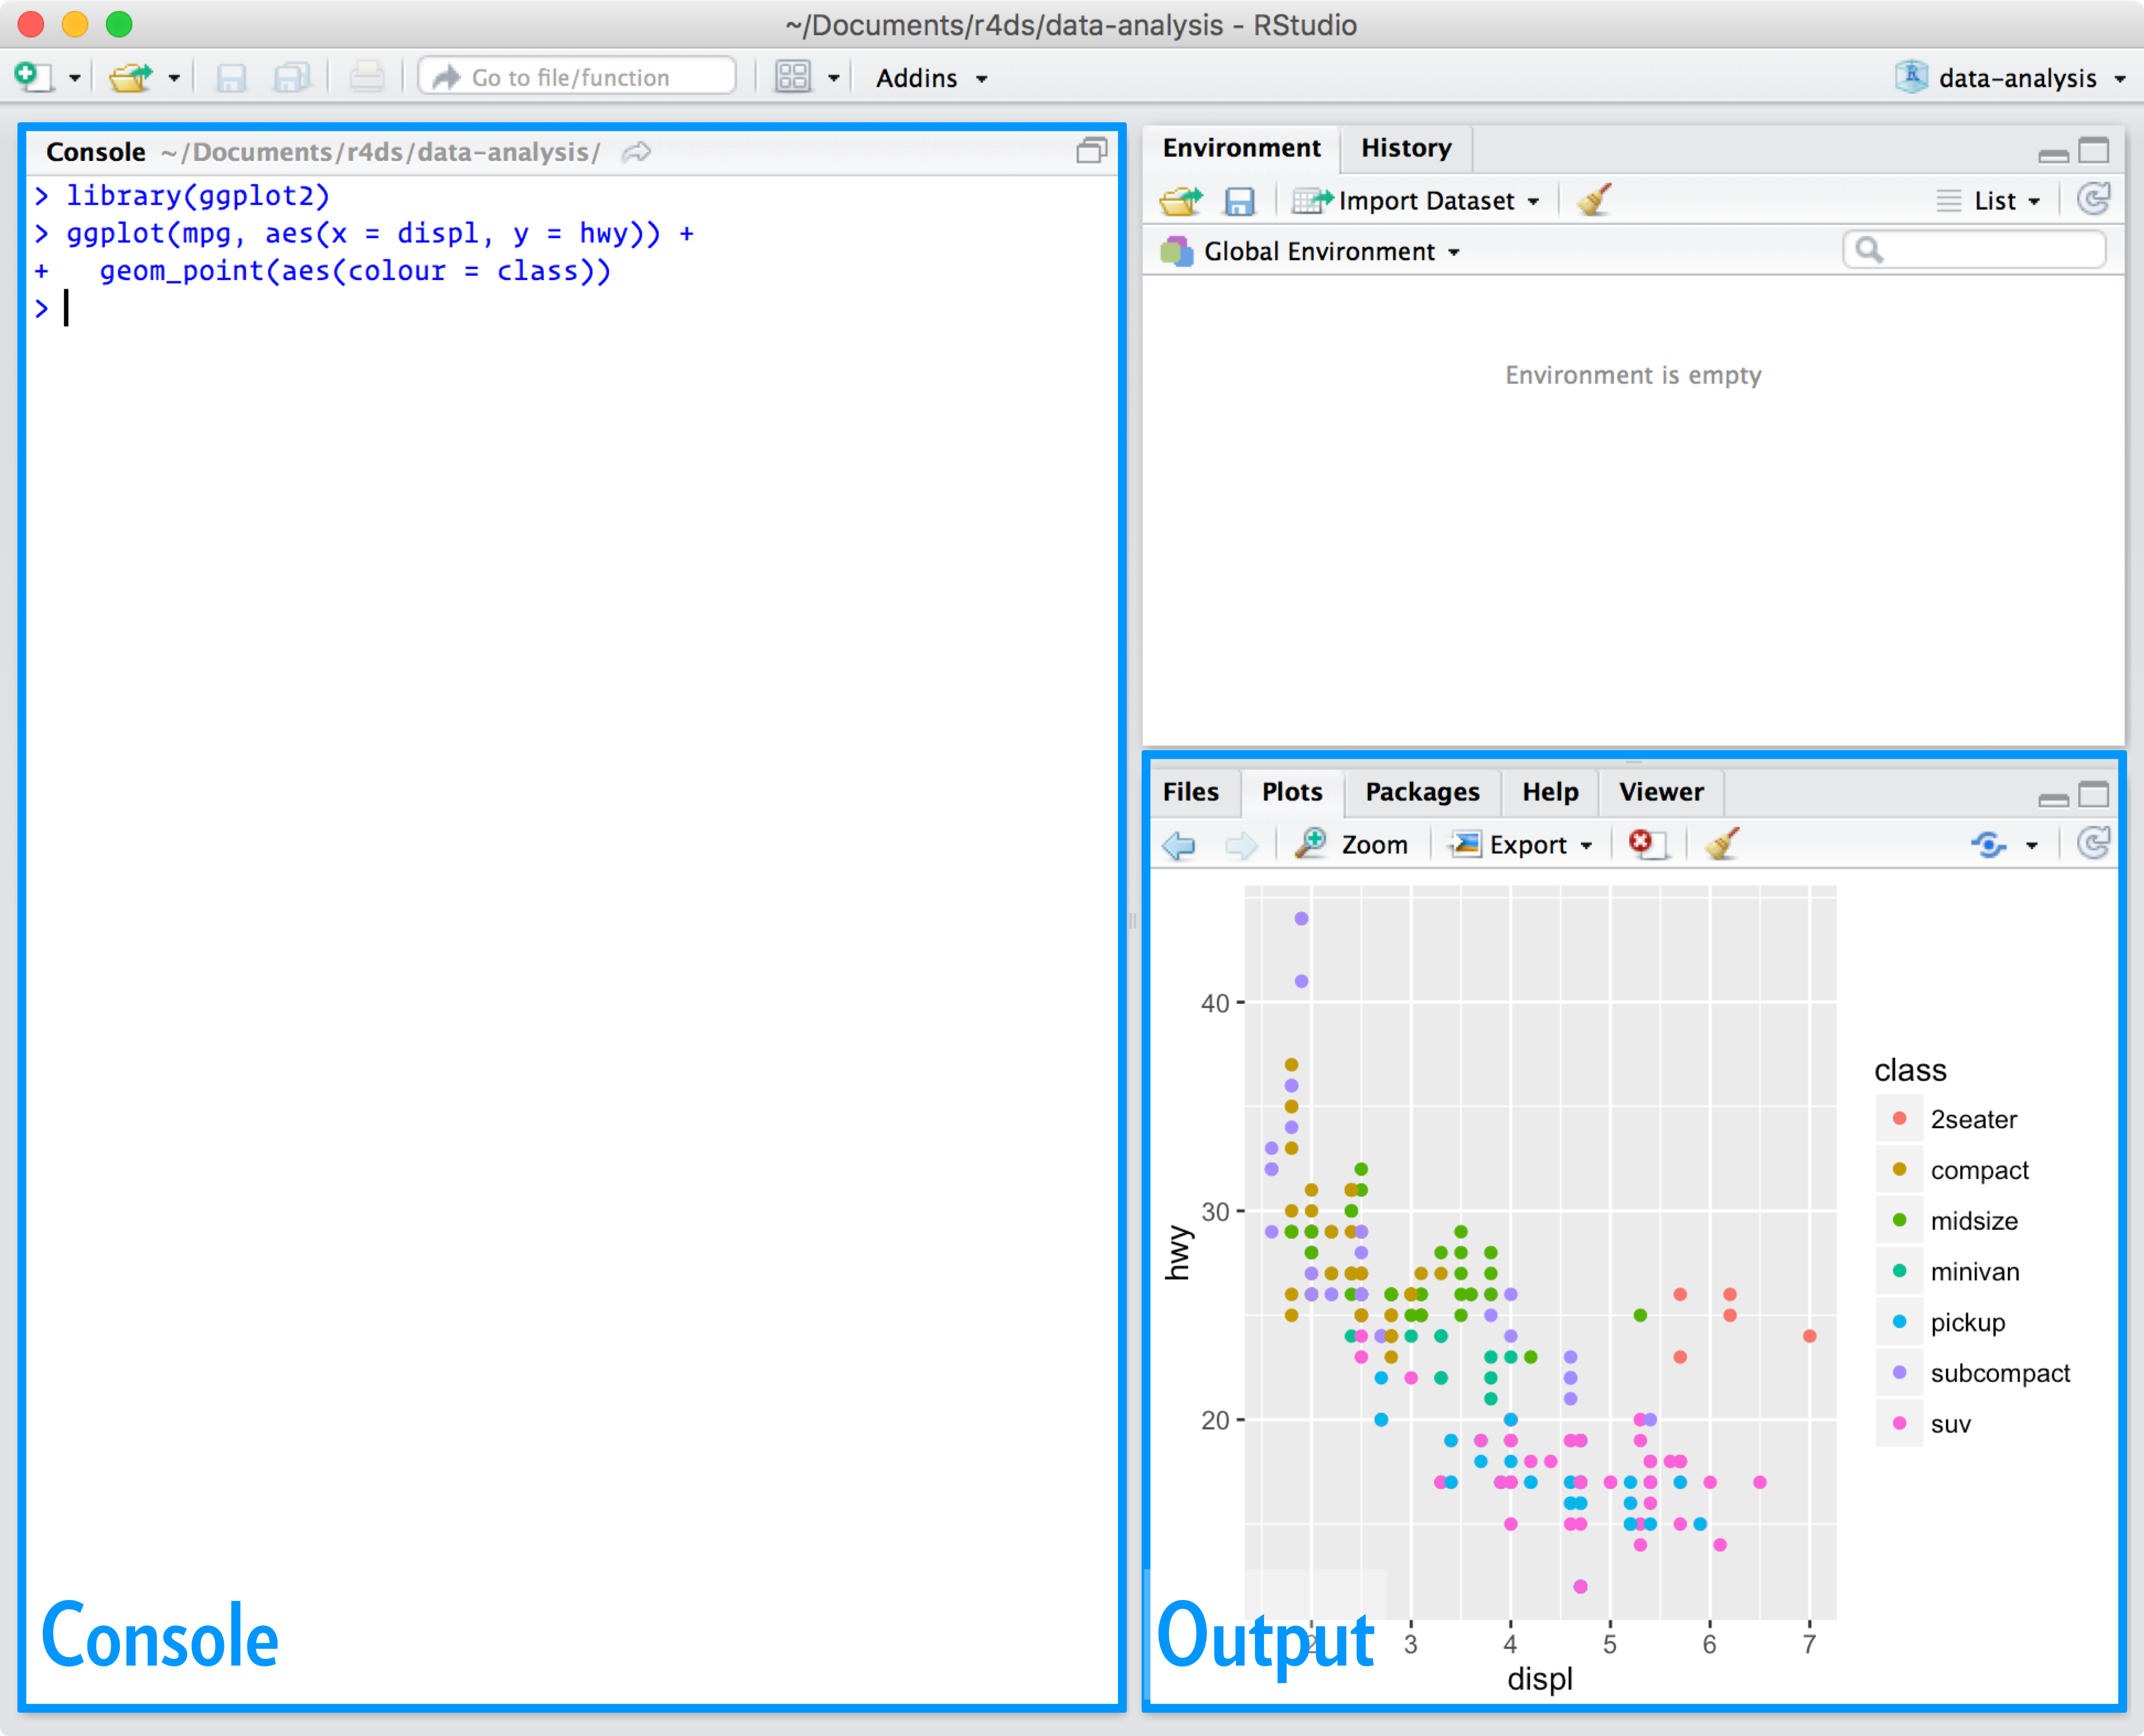
\includegraphics[width=0.9\linewidth]{images/rstudio-console} \end{center}

You can type R code into the \emph{Console} part of the interface and
press the enter key to run the code.

\subsection{R packages}\label{r-packages}

An R package is a collection of R code and documentation that can be
installed to enhance the standard R environment with additional
functionality. Currently, there are over ten thousand R packages
available on CRAN. Each of these R packages (mostly) aim to serve a
specific need, such as
\href{https://cran.r-project.org/web/packages/readxl/index.html}{reading
Excel spreadsheets},
\href{https://cran.r-project.org/web/packages/MODIStsp/index.html}{downloading
satellite imagery data},
\href{https://cran.r-project.org/web/packages/wdpar/index.html}{downloading
and cleaning protected area data}, or
\href{https://cran.r-project.org/web/packages/ENMeval/index.html}{fitting
environmental niche models}. In fact, R has such a diverse ecosystem of
R packages, that the question is (generally) not ``can I use R to do
\ldots{}?'' but ``what R package can I use to \ldots{}?''. During this
workshop, we will use various R packages. To install these R packages,
please run enter the code below in the \emph{Console} part of the
RStudio interface and press enter. Please note that you will require an
internet connection to install the packages and the installation process
may take a while to complete.

\begin{Shaded}
\begin{Highlighting}[]
\KeywordTok{install.packages}\NormalTok{(}\KeywordTok{c}\NormalTok{(}\StringTok{"sf"}\NormalTok{, }\StringTok{"tidyverse"}\NormalTok{, }\StringTok{"sp"}\NormalTok{, }\StringTok{"rgeos"}\NormalTok{, }\StringTok{"rgdal"}\NormalTok{, }\StringTok{"raster"}\NormalTok{, }\StringTok{"units"}\NormalTok{,}
                   \StringTok{"prioritizr"}\NormalTok{, }\StringTok{"prioritizrdata"} \StringTok{"Rsymphony"}\NormalTok{, }\StringTok{"mapview"}\NormalTok{,}
                   \StringTok{"assertthat"}\NormalTok{, }\StringTok{"velox"}\NormalTok{, }\StringTok{"remotes"}\NormalTok{, }\StringTok{"gridExtra"}\NormalTok{))}
\NormalTok{remotes}\OperatorTok{::}\KeywordTok{install_bioc}\NormalTok{(}\StringTok{"lpsymphony"}\NormalTok{)}
\end{Highlighting}
\end{Shaded}

\section{Further reading}\label{further-reading}

There is a wealth of resources available for learning how to use R.
Although not required for this workshop, I would highly recommend that
you read \href{https://r4ds.had.co.nz/}{\emph{R for Data Science} by
Garrett Grolemund and Hadley Wickham}. \textbf{This veritable trove of R
goodness is freely available online.} If you spend a week going through
this book then you will save months debugging and rerunning incorrect
code. I would urge any and all ecologists -- especially those working on
Masters or PhD degrees -- to read this book. I even bought this book as
a Christmas present for my sister---and, yes, she was happy to receive
it! For intermediate users looking to skill-up, I would recommend the
\href{http://shop.oreilly.com/product/9781593273842.do}{\emph{The Art of
R Programming: A Tour of Statistical Software Design} by Norman Matloff}
and \href{https://adv-r.hadley.nz/}{\emph{Advanced R} by Hadley
Wickham}. Finally, if you wish to learn more about using R as a
geospatial information system (GIS), I would recommend
\href{https://geocompr.robinlovelace.net/}{\emph{Geocomputation with R}
by Robin Lovelace, Jakub Nowosad, and Jannes Muenchow} which is also
freely available online. I also recommend
\href{https://www.springer.com/gp/book/9781461476177}{\emph{Applied
Spatial Data Analysis} by Roger S. Bivand, Edzer Pebesma, and Virgilio
Gómez-Rubio} too.

\chapter{Data}\label{data}

\section{Starting out}\label{starting-out}

We will start by opening RStudio. Ideally, you will have already
installed both R and Rstudio before the workshop. If you have not done
this already, then please see the \protect\hyperlink{setup}{Setting up
your computer} section. \textbf{During this workshop, please do not copy
and paste code from the workshop manual into RStudio. Instead, please
write it out yourself in an R script.} When programming, you will spend
a lot of time fixing coding mistakes -- that is, debugging your code --
so it is best to get used to making mistakes now when you have people
here to help you. You can create a new R script by clicking on
\emph{File} in the RStudio menu bar and then \emph{R Script}.

\begin{center}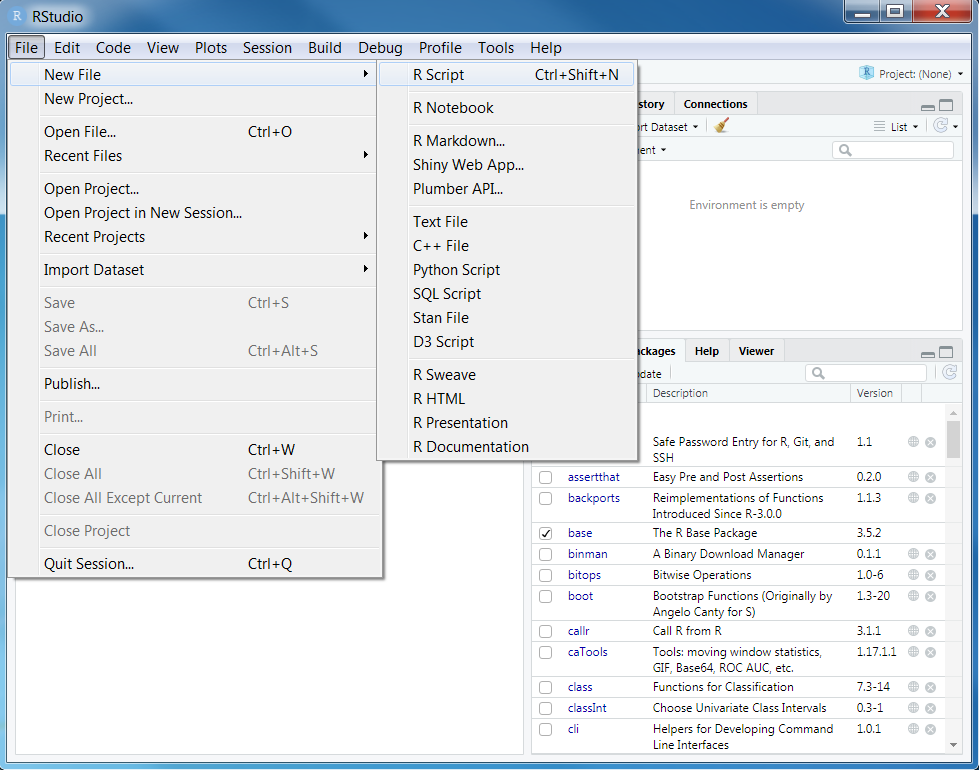
\includegraphics[width=0.7\linewidth]{images/rstudio-new-script} \end{center}

After creating a new script, you will notice that a new \emph{Source}
panel has appeared. In this new \emph{Source} panel, you can type and
edit code. You can run code in the \emph{Source} panel by placing the
cursor (i.e.~the blinking line) on the desired line of code and pressing
\texttt{Control\ +\ Enter} on your keyboard (or \texttt{CMD\ +\ Enter}
if you are using an Apple computer). You can save the code in the
\emph{Source} panel by pressing \texttt{Control\ +\ s} on your keyboard
(or \texttt{CMD\ +\ s} if you are using an Apple computer).

\begin{center}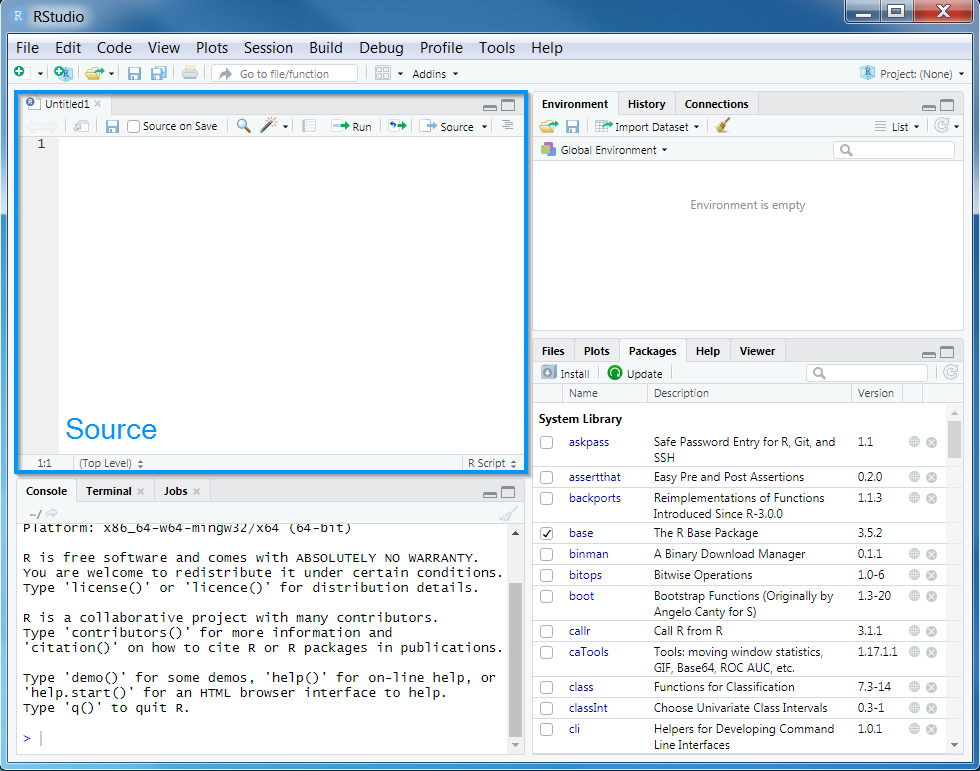
\includegraphics[width=0.7\linewidth]{images/rstudio-source} \end{center}

You can also make notes and write your answers to the workshop questions
inside the \emph{Source} panel. When writing notes and answers, add a
\texttt{\#} symbol so that the text following the \texttt{\#} symbol is
treated as a comment and not code. This means that you don't have to
worry about highlighting specific parts of the script to avoid errors.

\begin{Shaded}
\begin{Highlighting}[]
\CommentTok{# this is a comment and R will ignore this text if you run it}
\CommentTok{# R will run the code below because it does not start with a # symbol}
\KeywordTok{print}\NormalTok{(}\StringTok{"this is not a comment"}\NormalTok{)}
\end{Highlighting}
\end{Shaded}

\begin{verbatim}
## [1] "this is not a comment"
\end{verbatim}

\begin{Shaded}
\begin{Highlighting}[]
\CommentTok{# you can also add comments to the same line of R code too}
\KeywordTok{print}\NormalTok{(}\StringTok{"this is also not a comment"}\NormalTok{) }\CommentTok{# but this is a comment}
\end{Highlighting}
\end{Shaded}

\begin{verbatim}
## [1] "this is also not a comment"
\end{verbatim}

\textbf{Remember to save your script regularly to ensure that you don't
lose anything in the event that RStudio crashes (e.g.~using
\texttt{Control\ +\ s} or \texttt{CMD\ +\ s})!}

\section{Attaching packages}\label{attaching-packages}

Now we will setup our R session for the workshop. Specifically, enter
the following R code to attach the R packages used in this workshop.

\begin{Shaded}
\begin{Highlighting}[]
\CommentTok{# load packages}
\KeywordTok{library}\NormalTok{(tidyverse)}
\KeywordTok{library}\NormalTok{(prioritizr)}
\KeywordTok{library}\NormalTok{(rgdal)}
\KeywordTok{library}\NormalTok{(raster)}
\KeywordTok{library}\NormalTok{(rgeos)}
\KeywordTok{library}\NormalTok{(mapview)}
\KeywordTok{library}\NormalTok{(units)}
\KeywordTok{library}\NormalTok{(scales)}
\KeywordTok{library}\NormalTok{(assertthat)}
\KeywordTok{library}\NormalTok{(gridExtra)}
\end{Highlighting}
\end{Shaded}

You should have already downloaded the data for the prioritizr module of
this workshop. If you have not already done so, you can download it from
here:
\url{https://github.com/prioritizr/cibio-workshop/raw/master/data.zip}.
After downloading the data, you can unzip the data into a new folder.
Next, you will need to set the working directory to this new folder. To
achieve this, click on the \emph{Session} button on the RStudio menu
bar, then click \emph{Set working directory}, and then \emph{Choose
Directory}.

\begin{center}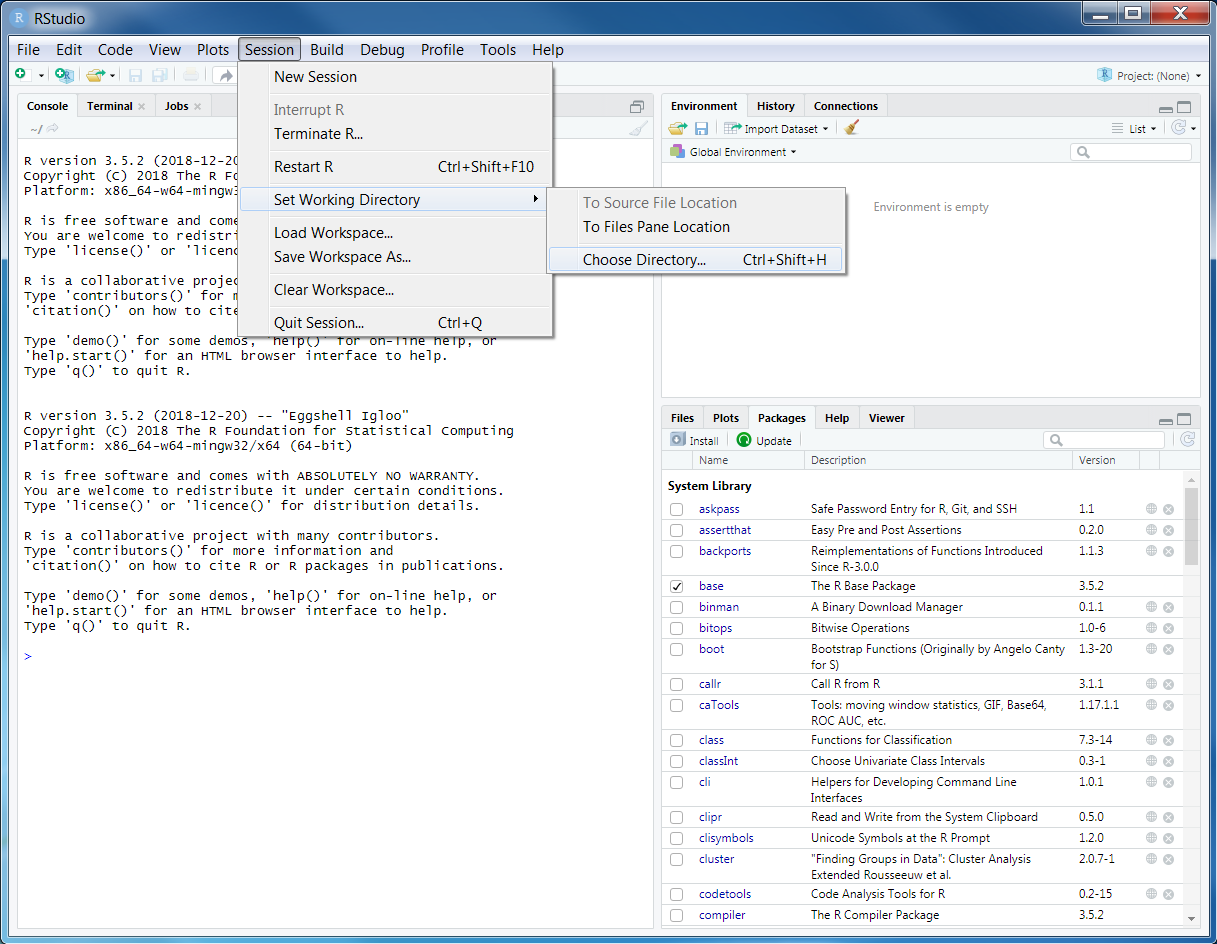
\includegraphics[width=0.7\linewidth]{images/rstudio-wd} \end{center}

Now navigate to the folder where you unzipped the data and select
\emph{Open}. You can verify that you have correctly set the working
directory using the following R code. You should see the output
\texttt{TRUE} in the \emph{Console} panel.

\begin{Shaded}
\begin{Highlighting}[]
\KeywordTok{file.exists}\NormalTok{(}\StringTok{"data/pu.shp"}\NormalTok{)}
\end{Highlighting}
\end{Shaded}

\begin{verbatim}
## [1] TRUE
\end{verbatim}

\section{Data import}\label{data-import}

Now that we have downloaded the dataset, we will need to import it into
our R session. Specifically, this data was obtained from the
``Introduction to Marxan'' course and was originally a subset of a
larger spatial prioritization project performed under contract to
Australia's Department of Environment and Water Resources. It contains
vector-based planning unit data (\texttt{pu.shp}) and the raster-based
data describing the spatial distributions of 62 vegetation classes
(\texttt{vegetation.tif}) in Tasmania, Australia. Please note this
dataset is only provided for teaching purposes and should not be used
for any real-world conservation planning. We can import the data into
our R session using the following code.

\begin{Shaded}
\begin{Highlighting}[]
\CommentTok{# import planning unit data}
\NormalTok{pu_data <-}\StringTok{ }\KeywordTok{readOGR}\NormalTok{(}\StringTok{"data/pu.shp"}\NormalTok{)}
\end{Highlighting}
\end{Shaded}

\begin{verbatim}
## OGR data source with driver: ESRI Shapefile 
## Source: "/home/travis/build/prioritizr/cibio-workshop/data/pu.shp", layer: "pu"
## with 1130 features
## It has 5 fields
\end{verbatim}

\begin{Shaded}
\begin{Highlighting}[]
\CommentTok{# format columns in planning unit data}
\NormalTok{pu_data}\OperatorTok{$}\NormalTok{locked_in <-}\StringTok{ }\KeywordTok{as.logical}\NormalTok{(pu_data}\OperatorTok{$}\NormalTok{locked_in)}
\NormalTok{pu_data}\OperatorTok{$}\NormalTok{locked_out <-}\StringTok{ }\KeywordTok{as.logical}\NormalTok{(pu_data}\OperatorTok{$}\NormalTok{locked_out)}

\CommentTok{# import vegetation data}
\NormalTok{veg_data <-}\StringTok{ }\KeywordTok{stack}\NormalTok{(}\StringTok{"data/vegetation.tif"}\NormalTok{)}
\end{Highlighting}
\end{Shaded}

\section{Planning unit data}\label{planning-unit-data}

The planning unit data contains spatial data describing the geometry for
each planning unit and attribute data with information about each
planning unit (e.g.~cost values). Let's investigate the
\texttt{pu\_data} object. The attribute data contains 5 columns with
contain the following information:

\begin{itemize}
\tightlist
\item
  \texttt{id}: unique identifiers for each planning unit
\item
  \texttt{cost}: acquisition cost values for each planning unit
  (millions of Australian dollars).
\item
  \texttt{status}: status information for each planning unit (only
  relevant with Marxan)
\item
  \texttt{locked\_in}: logical values (i.e.
  \texttt{TRUE}/\texttt{FALSE}) indicating if planning units are covered
  by protected areas or not.
\item
  \texttt{locked\_out}: logical values (i.e.
  \texttt{TRUE}/\texttt{FALSE}) indicating if planning units cannot be
  managed as a protected area because they contain too much
  anthropologically altered land.
\end{itemize}

\begin{Shaded}
\begin{Highlighting}[]
\CommentTok{# print a short summary of the data}
\KeywordTok{print}\NormalTok{(pu_data)}
\end{Highlighting}
\end{Shaded}

\begin{verbatim}
## class       : SpatialPolygonsDataFrame 
## features    : 1130 
## extent      : 1080623, 1399989, -4840595, -4497092  (xmin, xmax, ymin, ymax)
## crs         : +proj=aea +lat_1=-18 +lat_2=-36 +lat_0=0 +lon_0=132 +x_0=0 +y_0=0 +ellps=GRS80 +units=m +no_defs 
## variables   : 5
## names       :   id,              cost, status, locked_in, locked_out 
## min values  :    1, 0.192488262910798,      0,         0,          0 
## max values  : 1130,  61.9272727272727,      2,         1,          1
\end{verbatim}

\begin{Shaded}
\begin{Highlighting}[]
\CommentTok{# plot the planning unit data}
\KeywordTok{plot}\NormalTok{(pu_data)}
\end{Highlighting}
\end{Shaded}

\begin{center}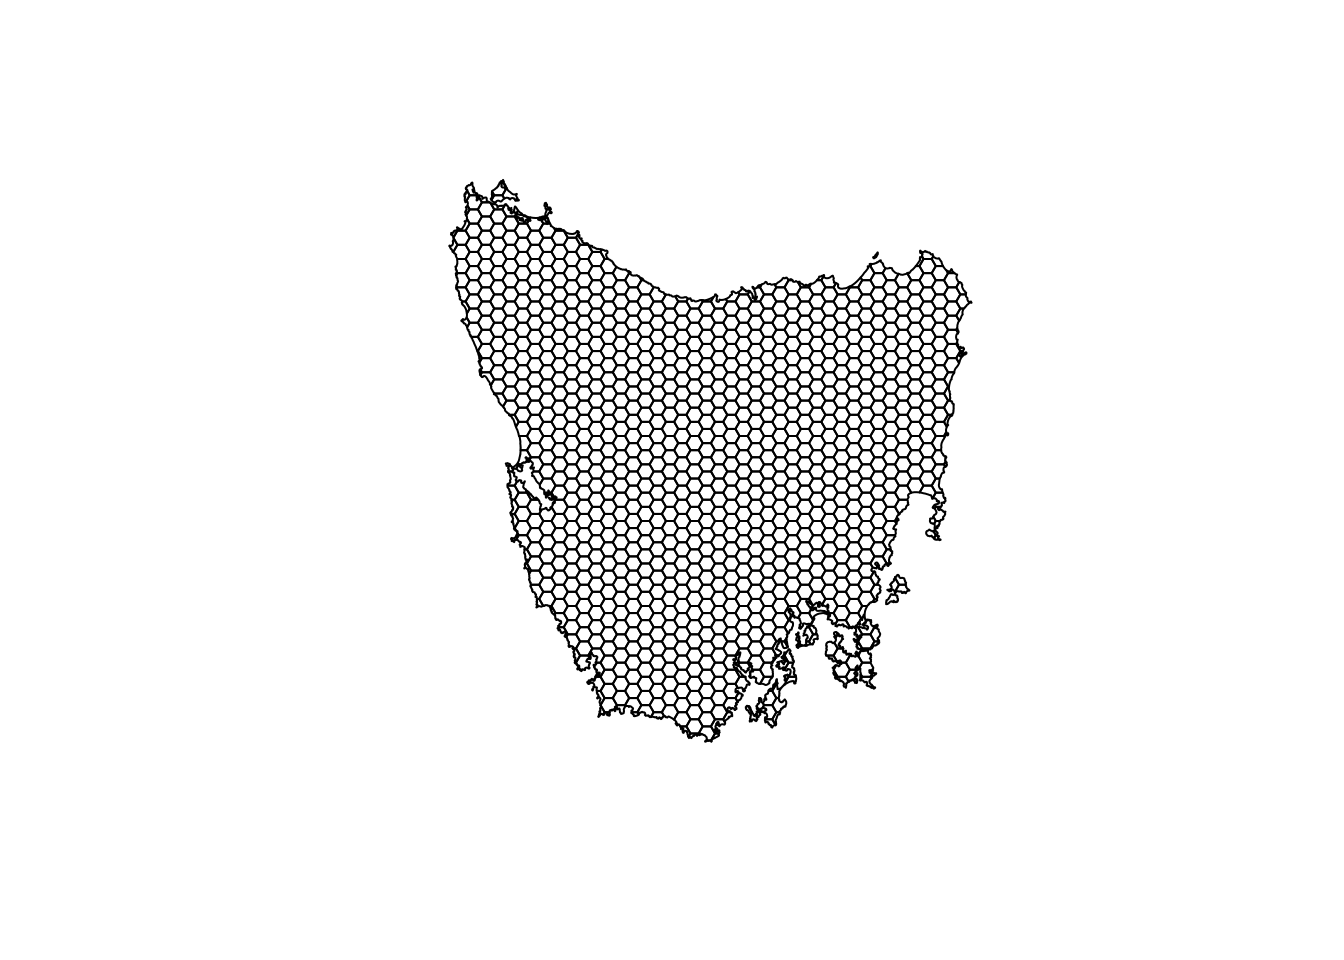
\includegraphics{prioritizr-workshop-manual_files/figure-latex/unnamed-chunk-15-1} \end{center}

\begin{Shaded}
\begin{Highlighting}[]
\CommentTok{# plot an interactive map of the planning unit data}
\KeywordTok{mapview}\NormalTok{(pu_data)}
\end{Highlighting}
\end{Shaded}

\begin{Shaded}
\begin{Highlighting}[]
\CommentTok{# print the structure of object}
\KeywordTok{str}\NormalTok{(pu_data, }\DataTypeTok{max.level =} \DecValTok{2}\NormalTok{)}
\end{Highlighting}
\end{Shaded}

\begin{verbatim}
## Formal class 'SpatialPolygonsDataFrame' [package "sp"] with 5 slots
##   ..@ data       :'data.frame':  1130 obs. of  5 variables:
##   ..@ polygons   :List of 1130
##   ..@ plotOrder  : int [1:1130] 217 973 506 645 705 975 253 271 704 889 ...
##   ..@ bbox       : num [1:2, 1:2] 1080623 -4840595 1399989 -4497092
##   .. ..- attr(*, "dimnames")=List of 2
##   ..@ proj4string:Formal class 'CRS' [package "sp"] with 1 slot
\end{verbatim}

\begin{Shaded}
\begin{Highlighting}[]
\CommentTok{# print the class of the object}
\KeywordTok{class}\NormalTok{(pu_data)}
\end{Highlighting}
\end{Shaded}

\begin{verbatim}
## [1] "SpatialPolygonsDataFrame"
## attr(,"package")
## [1] "sp"
\end{verbatim}

\begin{Shaded}
\begin{Highlighting}[]
\CommentTok{# print the slots of the object}
\KeywordTok{slotNames}\NormalTok{(pu_data)}
\end{Highlighting}
\end{Shaded}

\begin{verbatim}
## [1] "data"        "polygons"    "plotOrder"   "bbox"        "proj4string"
\end{verbatim}

\begin{Shaded}
\begin{Highlighting}[]
\CommentTok{# print the geometry for the 80th planning unit}
\NormalTok{pu_data}\OperatorTok{@}\NormalTok{polygons[[}\DecValTok{80}\NormalTok{]]}
\end{Highlighting}
\end{Shaded}

\begin{verbatim}
## An object of class "Polygons"
## Slot "Polygons":
## [[1]]
## An object of class "Polygon"
## Slot "labpt":
## [1]  1289177 -4558185
## 
## Slot "area":
## [1] 1060361
## 
## Slot "hole":
## [1] FALSE
## 
## Slot "ringDir":
## [1] 1
## 
## Slot "coords":
##          [,1]     [,2]
##  [1,] 1288123 -4558431
##  [2,] 1287877 -4558005
##  [3,] 1288177 -4558019
##  [4,] 1288278 -4558054
##  [5,] 1288834 -4558038
##  [6,] 1289026 -4557929
##  [7,] 1289168 -4557928
##  [8,] 1289350 -4557790
##  [9,] 1289517 -4557744
## [10,] 1289618 -4557773
## [11,] 1289836 -4557965
## [12,] 1290000 -4557984
## [13,] 1290025 -4557987
## [14,] 1290144 -4558168
## [15,] 1290460 -4558431
## [16,] 1288123 -4558431
## 
## 
## 
## Slot "plotOrder":
## [1] 1
## 
## Slot "labpt":
## [1]  1289177 -4558185
## 
## Slot "ID":
## [1] "79"
## 
## Slot "area":
## [1] 1060361
\end{verbatim}

\begin{Shaded}
\begin{Highlighting}[]
\CommentTok{# print the coordinate reference system}
\KeywordTok{print}\NormalTok{(pu_data}\OperatorTok{@}\NormalTok{proj4string)}
\end{Highlighting}
\end{Shaded}

\begin{verbatim}
## CRS arguments:
##  +proj=aea +lat_1=-18 +lat_2=-36 +lat_0=0 +lon_0=132 +x_0=0 +y_0=0
## +ellps=GRS80 +units=m +no_defs
\end{verbatim}

\begin{Shaded}
\begin{Highlighting}[]
\CommentTok{# print number of planning units (geometries) in the data}
\KeywordTok{nrow}\NormalTok{(pu_data)}
\end{Highlighting}
\end{Shaded}

\begin{verbatim}
## [1] 1130
\end{verbatim}

\begin{Shaded}
\begin{Highlighting}[]
\CommentTok{# print the first six rows in the attribute data}
\KeywordTok{head}\NormalTok{(pu_data}\OperatorTok{@}\NormalTok{data)}
\end{Highlighting}
\end{Shaded}

\begin{verbatim}
##   id     cost status locked_in locked_out
## 0  1 60.24638      0     FALSE       TRUE
## 1  2 19.86301      0     FALSE      FALSE
## 2  3 59.68051      0     FALSE       TRUE
## 3  4 32.41614      0     FALSE      FALSE
## 4  5 26.17706      0     FALSE      FALSE
## 5  6 51.26218      0     FALSE       TRUE
\end{verbatim}

\begin{Shaded}
\begin{Highlighting}[]
\CommentTok{# print the first six values in the cost column of the attribute data}
\KeywordTok{head}\NormalTok{(pu_data}\OperatorTok{$}\NormalTok{cost)}
\end{Highlighting}
\end{Shaded}

\begin{verbatim}
## [1] 60.24638 19.86301 59.68051 32.41614 26.17706 51.26218
\end{verbatim}

\begin{Shaded}
\begin{Highlighting}[]
\CommentTok{# print the highest cost value}
\KeywordTok{max}\NormalTok{(pu_data}\OperatorTok{$}\NormalTok{cost)}
\end{Highlighting}
\end{Shaded}

\begin{verbatim}
## [1] 61.92727
\end{verbatim}

\begin{Shaded}
\begin{Highlighting}[]
\CommentTok{# print the smallest cost value}
\KeywordTok{min}\NormalTok{(pu_data}\OperatorTok{$}\NormalTok{cost)}
\end{Highlighting}
\end{Shaded}

\begin{verbatim}
## [1] 0.1924883
\end{verbatim}

\begin{Shaded}
\begin{Highlighting}[]
\CommentTok{# print average cost value}
\KeywordTok{mean}\NormalTok{(pu_data}\OperatorTok{$}\NormalTok{cost)}
\end{Highlighting}
\end{Shaded}

\begin{verbatim}
## [1] 25.13536
\end{verbatim}

\begin{Shaded}
\begin{Highlighting}[]
\CommentTok{# plot a map of the planning unit cost data}
\KeywordTok{spplot}\NormalTok{(pu_data, }\StringTok{"cost"}\NormalTok{)}
\end{Highlighting}
\end{Shaded}

\begin{center}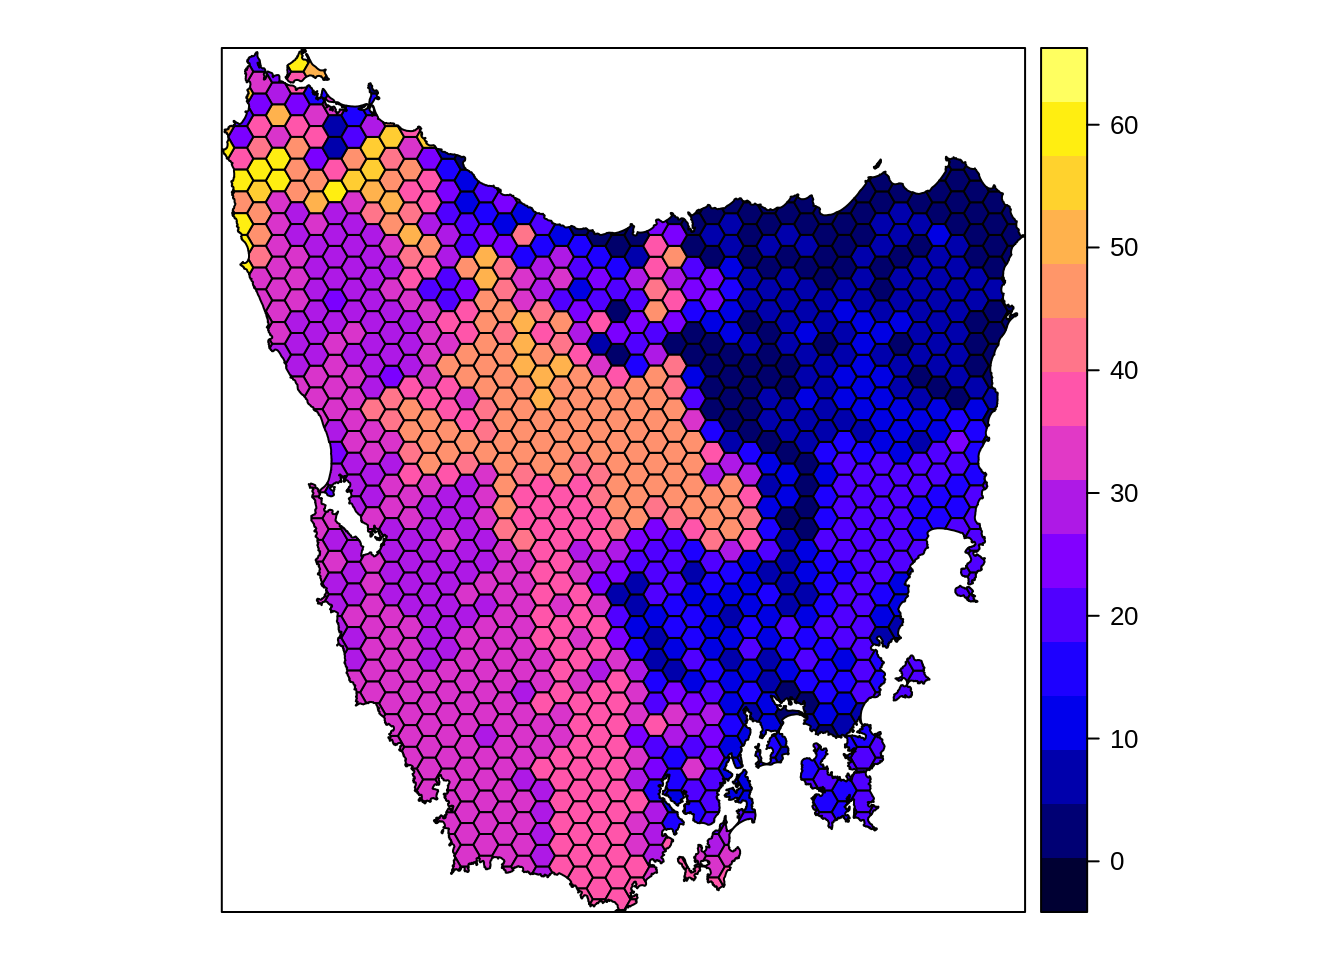
\includegraphics[width=0.6\linewidth]{prioritizr-workshop-manual_files/figure-latex/unnamed-chunk-17-1} \end{center}

\begin{Shaded}
\begin{Highlighting}[]
\CommentTok{# plot an interactive map of the planning unit cost data}
\KeywordTok{mapview}\NormalTok{(pu_data, }\DataTypeTok{zcol =} \StringTok{"cost"}\NormalTok{)}
\end{Highlighting}
\end{Shaded}

Now, you can try and answer some questions about the planning unit data.

\BeginKnitrBlock{rmdquestion}
\begin{enumerate}
\def\labelenumi{\arabic{enumi}.}
\tightlist
\item
  How many planning units are in the planning unit data?
\item
  What is the highest cost value?
\item
  How many planning units are covered by the protected areas (hint:
  \texttt{sum(x)})?
\item
  What is the proportion of the planning units that are covered by the
  protected areas (hint: \texttt{mean(x)})?
\item
  How many planning units are dominated by anthropologically altered
  land (hint: \texttt{sum(x)})?
\item
  What is the proportion of planning units dominated by
  anthropologically altered land (hint: \texttt{mean(x)})?
\item
  Can you verify that all values in the \texttt{locked\_in} and
  \texttt{locked\_out} columns are zero or one (hint: \texttt{min(x)}
  and \texttt{max(x)})?.
\item
  Can you verify that none of the planning units are missing cost values
  (hint: \texttt{all(is.finite(x))})?.
\item
  Can you very that none of the planning units have duplicated
  identifiers? (hint: \texttt{sum(duplicated(x))})?
\item
  Is there a spatial pattern in the planning unit cost values (hint: use
  \texttt{spplot} to make a map).
\item
  Is there a spatial pattern in where most planning units are covered by
  protected areas (hint: use \texttt{spplot} to make a map).
\end{enumerate}
\EndKnitrBlock{rmdquestion}

\clearpage

\section{Vegetation data}\label{vegetation-data}

The vegetation data describes the spatial distribution of 62 vegetation
classes in the study area. This data is in a raster format and so the
data are organized using a regular spatial grid with square grid cells.
In our case, our raster data contains multiple layers (also called
``bands'') and each layer has corresponds to a spatial grid with exactly
the same area and has exactly the same dimensionality (i.e.~number of
rows, columns, and cells). In this dataset, there are 62 different
regular spatial grids layered on top of each other -- with each layer
corresponding to a different vegetation class -- and each of these
layers contains a grid with 343 columns, 320 rows, and 109760 cells.
Within each layer, each cell corresponds to a 1 by 1 km square. The
values associated with each grid cell contain values (i.e.~one or zero)
indicating the presence or absence of a given vegetation class in the
cell.

\begin{figure}
\centering
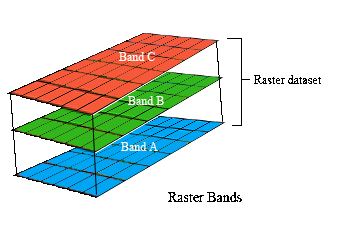
\includegraphics{images/rasterbands.png}
\caption{}
\end{figure}

Let's explore the vegetation data.

\begin{Shaded}
\begin{Highlighting}[]
\CommentTok{# print a short summary of the data}
\KeywordTok{print}\NormalTok{(veg_data)}
\end{Highlighting}
\end{Shaded}

\begin{verbatim}
## class      : RasterStack 
## dimensions : 343, 320, 109760, 62  (nrow, ncol, ncell, nlayers)
## resolution : 1000, 1000  (x, y)
## extent     : 1080496, 1400496, -4841217, -4498217  (xmin, xmax, ymin, ymax)
## crs        : +proj=aea +lat_1=-18 +lat_2=-36 +lat_0=0 +lon_0=132 +x_0=0 +y_0=0 +ellps=GRS80 +units=m +no_defs 
## names      : vegetation.1, vegetation.2, vegetation.3, vegetation.4, vegetation.5, vegetation.6, vegetation.7, vegetation.8, vegetation.9, vegetation.10, vegetation.11, vegetation.12, vegetation.13, vegetation.14, vegetation.15, ... 
## min values :            0,            0,            0,            0,            0,            0,            0,            0,            0,             0,             0,             0,             0,             0,             0, ... 
## max values :            1,            1,            1,            1,            1,            1,            1,            1,            1,             1,             1,             1,             1,             1,             1, ...
\end{verbatim}

\begin{Shaded}
\begin{Highlighting}[]
\CommentTok{# plot a map of the 36th vegetation class}
\KeywordTok{plot}\NormalTok{(veg_data[[}\DecValTok{36}\NormalTok{]])}
\end{Highlighting}
\end{Shaded}

\begin{center}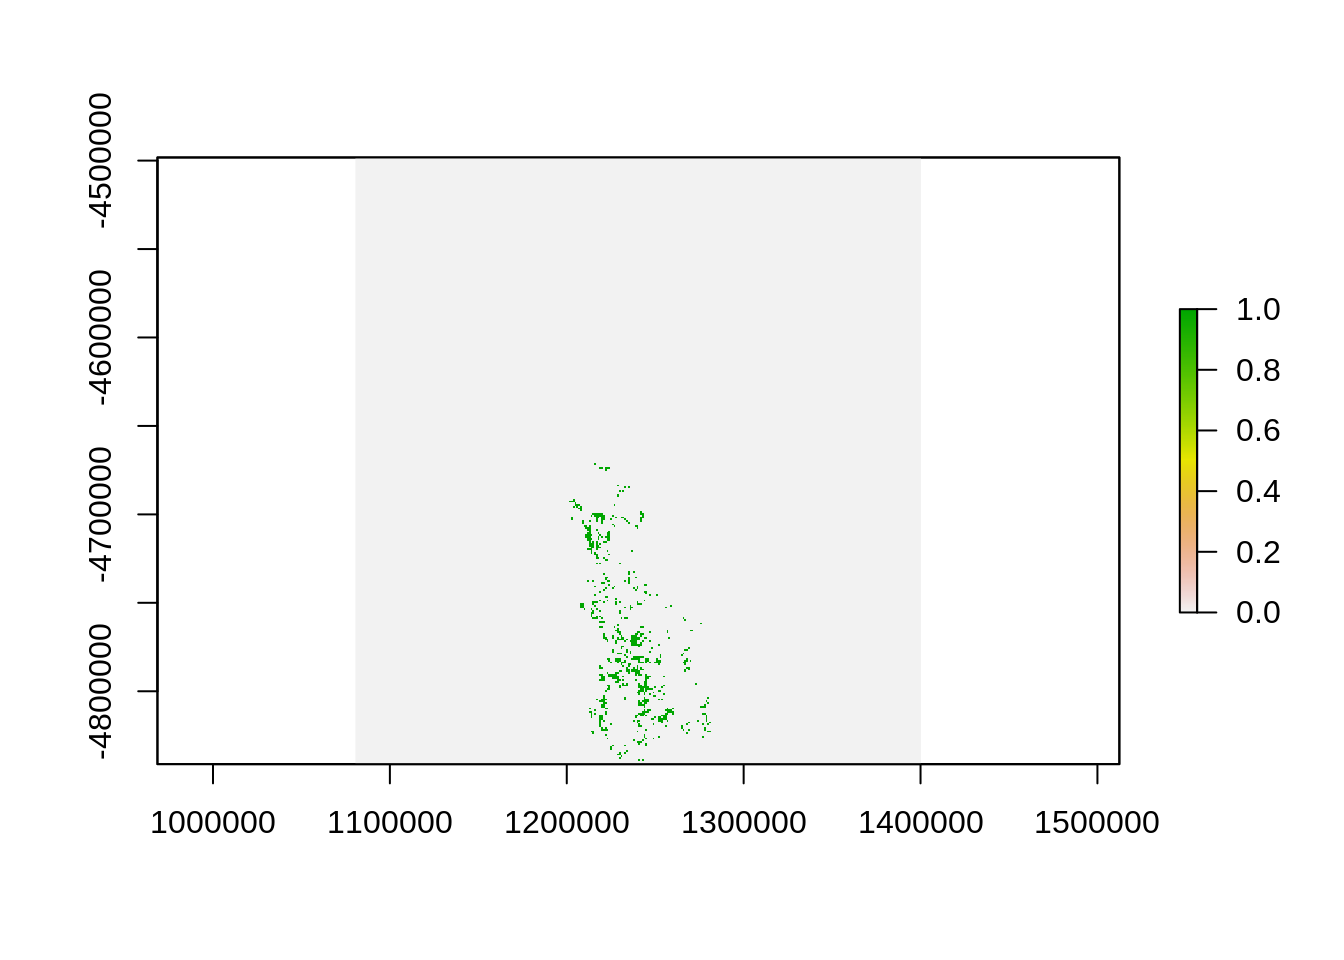
\includegraphics{prioritizr-workshop-manual_files/figure-latex/unnamed-chunk-20-1} \end{center}

\begin{Shaded}
\begin{Highlighting}[]
\CommentTok{# plot an interactive map of the 36th vegetation class}
\KeywordTok{mapview}\NormalTok{(veg_data[[}\DecValTok{36}\NormalTok{]])}
\end{Highlighting}
\end{Shaded}

\begin{Shaded}
\begin{Highlighting}[]
\CommentTok{# print number of rows in the data}
\KeywordTok{nrow}\NormalTok{(veg_data)}
\end{Highlighting}
\end{Shaded}

\begin{verbatim}
## [1] 343
\end{verbatim}

\begin{Shaded}
\begin{Highlighting}[]
\CommentTok{# print number of columns  in the data}
\KeywordTok{ncol}\NormalTok{(veg_data)}
\end{Highlighting}
\end{Shaded}

\begin{verbatim}
## [1] 320
\end{verbatim}

\begin{Shaded}
\begin{Highlighting}[]
\CommentTok{# print number of cells in the data}
\KeywordTok{ncell}\NormalTok{(veg_data)}
\end{Highlighting}
\end{Shaded}

\begin{verbatim}
## [1] 109760
\end{verbatim}

\begin{Shaded}
\begin{Highlighting}[]
\CommentTok{# print number of layers in the data}
\KeywordTok{nlayers}\NormalTok{(veg_data)}
\end{Highlighting}
\end{Shaded}

\begin{verbatim}
## [1] 62
\end{verbatim}

\begin{Shaded}
\begin{Highlighting}[]
\CommentTok{# print  resolution on the x-axis}
\KeywordTok{xres}\NormalTok{(veg_data)}
\end{Highlighting}
\end{Shaded}

\begin{verbatim}
## [1] 1000
\end{verbatim}

\begin{Shaded}
\begin{Highlighting}[]
\CommentTok{# print resolution on the y-axis}
\KeywordTok{yres}\NormalTok{(veg_data)}
\end{Highlighting}
\end{Shaded}

\begin{verbatim}
## [1] 1000
\end{verbatim}

\begin{Shaded}
\begin{Highlighting}[]
\CommentTok{# print spatial extent of the grid, i.e. coordinates for corners}
\KeywordTok{extent}\NormalTok{(veg_data)}
\end{Highlighting}
\end{Shaded}

\begin{verbatim}
## class      : Extent 
## xmin       : 1080496 
## xmax       : 1400496 
## ymin       : -4841217 
## ymax       : -4498217
\end{verbatim}

\begin{Shaded}
\begin{Highlighting}[]
\CommentTok{# print the coordinate reference system}
\KeywordTok{print}\NormalTok{(veg_data}\OperatorTok{@}\NormalTok{crs)}
\end{Highlighting}
\end{Shaded}

\begin{verbatim}
## CRS arguments:
##  +proj=aea +lat_1=-18 +lat_2=-36 +lat_0=0 +lon_0=132 +x_0=0 +y_0=0
## +ellps=GRS80 +units=m +no_defs
\end{verbatim}

\begin{Shaded}
\begin{Highlighting}[]
\CommentTok{# print a summary of the first layer in the stack}
\KeywordTok{print}\NormalTok{(veg_data[[}\DecValTok{1}\NormalTok{]])}
\end{Highlighting}
\end{Shaded}

\begin{verbatim}
## class      : RasterLayer 
## band       : 1  (of  62  bands)
## dimensions : 343, 320, 109760  (nrow, ncol, ncell)
## resolution : 1000, 1000  (x, y)
## extent     : 1080496, 1400496, -4841217, -4498217  (xmin, xmax, ymin, ymax)
## crs        : +proj=aea +lat_1=-18 +lat_2=-36 +lat_0=0 +lon_0=132 +x_0=0 +y_0=0 +ellps=GRS80 +units=m +no_defs 
## source     : /home/travis/build/prioritizr/cibio-workshop/data/vegetation.tif 
## names      : vegetation.1 
## values     : 0, 1  (min, max)
\end{verbatim}

\begin{Shaded}
\begin{Highlighting}[]
\CommentTok{# print the value in the 800th cell in the first layer of the stack}
\KeywordTok{print}\NormalTok{(veg_data[[}\DecValTok{1}\NormalTok{]][}\DecValTok{800}\NormalTok{])}
\end{Highlighting}
\end{Shaded}

\begin{verbatim}
##   
## 0
\end{verbatim}

\begin{Shaded}
\begin{Highlighting}[]
\CommentTok{# print the value of the cell located in the 30th row and the 60th column of}
\CommentTok{# the first layer}
\KeywordTok{print}\NormalTok{(veg_data[[}\DecValTok{1}\NormalTok{]][}\DecValTok{30}\NormalTok{, }\DecValTok{60}\NormalTok{])}
\end{Highlighting}
\end{Shaded}

\begin{verbatim}
##   
## 0
\end{verbatim}

\begin{Shaded}
\begin{Highlighting}[]
\CommentTok{# calculate the sum of all the cell values in the first layer}
\KeywordTok{cellStats}\NormalTok{(veg_data[[}\DecValTok{1}\NormalTok{]], }\StringTok{"sum"}\NormalTok{)}
\end{Highlighting}
\end{Shaded}

\begin{verbatim}
## [1] 36
\end{verbatim}

\begin{Shaded}
\begin{Highlighting}[]
\CommentTok{# calculate the maximum value of all the cell values in the first layer}
\KeywordTok{cellStats}\NormalTok{(veg_data[[}\DecValTok{1}\NormalTok{]], }\StringTok{"max"}\NormalTok{)}
\end{Highlighting}
\end{Shaded}

\begin{verbatim}
## [1] 1
\end{verbatim}

\begin{Shaded}
\begin{Highlighting}[]
\CommentTok{# calculate the minimum value of all the cell values in the first layer}
\KeywordTok{cellStats}\NormalTok{(veg_data[[}\DecValTok{1}\NormalTok{]], }\StringTok{"min"}\NormalTok{)}
\end{Highlighting}
\end{Shaded}

\begin{verbatim}
## [1] 0
\end{verbatim}

\begin{Shaded}
\begin{Highlighting}[]
\CommentTok{# calculate the mean value of all the cell values in the first layer}
\KeywordTok{cellStats}\NormalTok{(veg_data[[}\DecValTok{1}\NormalTok{]], }\StringTok{"mean"}\NormalTok{)}
\end{Highlighting}
\end{Shaded}

\begin{verbatim}
## [1] 0.0003279883
\end{verbatim}

\clearpage

\begin{Shaded}
\begin{Highlighting}[]
\CommentTok{# calculate the maximum value in each layer}
\KeywordTok{as_tibble}\NormalTok{(}\KeywordTok{data.frame}\NormalTok{(}\DataTypeTok{max =} \KeywordTok{cellStats}\NormalTok{(veg_data, }\StringTok{"max"}\NormalTok{)))}
\end{Highlighting}
\end{Shaded}

\begin{verbatim}
## # A tibble: 62 x 1
##      max
##    <dbl>
##  1     1
##  2     1
##  3     1
##  4     1
##  5     1
##  6     1
##  7     1
##  8     1
##  9     1
## 10     1
## # ... with 52 more rows
\end{verbatim}

Now, you can try and answer some questions about the vegetation data.

\BeginKnitrBlock{rmdquestion}
\begin{enumerate}
\def\labelenumi{\arabic{enumi}.}
\tightlist
\item
  What part of the study area is the 51st vegetation class found in
  (hint: make a map)?
\item
  What proportion of cells contain the 12th vegetation class?
\item
  Which vegetation class is present in the greatest number of cells?
\end{enumerate}
\EndKnitrBlock{rmdquestion}

\chapter{Gap analysis}\label{gap-analysis}

\section{Introduction}\label{introduction-1}

Before we begin to prioritize areas for protected area establishment, we
should first understand how well existing protected areas are conserving
our biodiversity features (i.e.~native vegetation classes in Tasmania,
Australia). This step is critical: we cannot develop plans to improve
conservation of biodiversity if we don't understand how well existing
policies are currently conserving biodiversity! To achieve this, we can
perform a ``gap analysis''. A gap analysis involves calculating how well
each of our biodiversity features (i.e.~vegetation classes in this
exercise) are represented (covered) by protected areas. Next, we compare
current representation by protected areas of each feature (e.g.~5\% of
their spatial distribution covered by protected areas) to a target
threshold (e.g.~20\% of their spatial distribution covered by protected
areas). This target threshold denotes the minimum amount (e.g.~minimum
proportion of spatial distribution) that we need of each feature to be
represented in the protected area system. Ideally, targets should be
based on an estimate of how much area or habitat is needed for ecosystem
function or species persistence. In practice, targets are generally set
using simple rules of thumb (e.g.~10\% or 20\%), policy (17\%;
\url{https://www.cbd.int/sp/targets/rationale/target-11}) or standard
practices \citep[e.g.~setting targets for species based on
range-size;][]{r1, r2}.

\section{Feature abundance}\label{feature-abundance}

Now we will perform some preliminary calculations for the gap analysis.
First, we will calculate how much of each vegetation feature occurs
inside each planning unit (i.e.~the abundance of the features). To
achieve this, we will use the \texttt{problem} function to create an
empty conservation planning problem that only contains the planning unit
and biodiversity data. We will then use the \texttt{feature\_abundances}
function to calculate the total amount of each feature in each planning
unit.

\begin{Shaded}
\begin{Highlighting}[]
\CommentTok{# create prioritizr problem with only the data}
\NormalTok{p0 <-}\StringTok{ }\KeywordTok{problem}\NormalTok{(pu_data, veg_data, }\DataTypeTok{cost_column =} \StringTok{"cost"}\NormalTok{)}

\CommentTok{# print empty problem,}
\CommentTok{# we can see that only the cost and feature data are defined}
\KeywordTok{print}\NormalTok{(p0)}
\end{Highlighting}
\end{Shaded}

\begin{verbatim}
## Conservation Problem
##   planning units: SpatialPolygonsDataFrame (1130 units)
##   cost:           min: 0.19249, max: 61.92727
##   features:       vegetation.1, vegetation.2, vegetation.3, ... (62 features)
##   objective:      none
##   targets:        none
##   decisions:      default
##   constraints:    <none>
##   penalties:      <none>
##   portfolio:      default
##   solver:         default
\end{verbatim}

\begin{Shaded}
\begin{Highlighting}[]
\CommentTok{# calculate amount of each feature in each planning unit}
\NormalTok{abundance_data <-}\StringTok{ }\KeywordTok{feature_abundances}\NormalTok{(p0)}

\CommentTok{# print abundance data}
\KeywordTok{print}\NormalTok{(abundance_data)}
\end{Highlighting}
\end{Shaded}

\begin{verbatim}
## # A tibble: 62 x 3
##    feature       absolute_abundance relative_abundance
##    <chr>                      <dbl>              <dbl>
##  1 vegetation.1                  33                  1
##  2 vegetation.2                 173                  1
##  3 vegetation.3                  24                  1
##  4 vegetation.4                  31                  1
##  5 vegetation.5                  23                  1
##  6 vegetation.6                  22                  1
##  7 vegetation.7                  15                  1
##  8 vegetation.8                  45                  1
##  9 vegetation.9                 384                  1
## 10 vegetation.10                 14                  1
## # ... with 52 more rows
\end{verbatim}

\clearpage

\begin{Shaded}
\begin{Highlighting}[]
\CommentTok{# note that only the first ten rows are printed,}
\CommentTok{# this is because the abundance_data object is a tibble (i.e. tbl_df) object}
\CommentTok{# and not a standard data.frame object}
\KeywordTok{print}\NormalTok{(}\KeywordTok{class}\NormalTok{(abundance_data))}
\end{Highlighting}
\end{Shaded}

\begin{verbatim}
## [1] "tbl_df"     "tbl"        "data.frame"
\end{verbatim}

\begin{Shaded}
\begin{Highlighting}[]
\CommentTok{# we can print all of the rows in abundance_data like this}
\KeywordTok{print}\NormalTok{(abundance_data, }\DataTypeTok{n =} \OtherTok{Inf}\NormalTok{)}
\end{Highlighting}
\end{Shaded}

\begin{verbatim}
## # A tibble: 62 x 3
##    feature       absolute_abundance relative_abundance
##    <chr>                      <dbl>              <dbl>
##  1 vegetation.1                  33                  1
##  2 vegetation.2                 173                  1
##  3 vegetation.3                  24                  1
##  4 vegetation.4                  31                  1
##  5 vegetation.5                  23                  1
##  6 vegetation.6                  22                  1
##  7 vegetation.7                  15                  1
##  8 vegetation.8                  45                  1
##  9 vegetation.9                 384                  1
## 10 vegetation.10                 14                  1
## 11 vegetation.11                 39                  1
## 12 vegetation.12                 26                  1
## 13 vegetation.13                 20                  1
## 14 vegetation.14                123                  1
## 15 vegetation.15                 18                  1
## 16 vegetation.16                 11                  1
## 17 vegetation.17                 24                  1
## 18 vegetation.18                 19                  1
## 19 vegetation.19                 24                  1
## 20 vegetation.20                895                  1
## 21 vegetation.21                258                  1
## 22 vegetation.22                  8                  1
## 23 vegetation.23                 10                  1
## 24 vegetation.24                 21                  1
## 25 vegetation.25                 13                  1
## 26 vegetation.26                  9                  1
## 27 vegetation.27                 15                  1
## 28 vegetation.28                660                  1
## 29 vegetation.29                 30                  1
## 30 vegetation.30                 26                  1
## 31 vegetation.31                 52                  1
## 32 vegetation.32                 30                  1
## 33 vegetation.33                312                  1
## 34 vegetation.34                 36                  1
## 35 vegetation.35                173                  1
## 36 vegetation.36                714                  1
## 37 vegetation.37                 26                  1
## 38 vegetation.38                 17                  1
## 39 vegetation.39                 18                  1
## 40 vegetation.40                 28                  1
## 41 vegetation.41                 59                  1
## 42 vegetation.42                  9                  1
## 43 vegetation.43                 80                  1
## 44 vegetation.44                139                  1
## 45 vegetation.45                 40                  1
## 46 vegetation.46                 25                  1
## 47 vegetation.47                 24                  1
## 48 vegetation.48                224                  1
## 49 vegetation.49                  4                  1
## 50 vegetation.50                 41                  1
## 51 vegetation.51                223                  1
## 52 vegetation.52                  2                  1
## 53 vegetation.53                  4                  1
## 54 vegetation.54                  5                  1
## 55 vegetation.55                  7                  1
## 56 vegetation.56                  8                  1
## 57 vegetation.57                 18                  1
## 58 vegetation.58                  4                  1
## 59 vegetation.59                 36                  1
## 60 vegetation.60                  2                  1
## 61 vegetation.61                  0                NaN
## 62 vegetation.62                  1                  1
\end{verbatim}

The \texttt{abundance\_data} object contains three columns. The
\texttt{feature} column contains the name of each feature (derived from
\texttt{names(veg\_data})), the \texttt{absolute\_abundance} column
contains the total amount of each feature in all the planning units, and
the \texttt{relative\_abundance} column contains the total amount of
each feature in the planning units expressed as a proportion of the
total amount in the underlying raster data. Since all the raster cells
containing vegetation overlap with the planning units, all of the values
in the \texttt{relative\_abundance} column are equal to one (meaning
100\%)---except for the 61st feature which has a value on \texttt{NaN}
because it does not occur in the study area at all (i.e.~all of its
raster values are zeros). Now let's add a new column with the feature
abundances expressed in aerial units (i.e.~km\textsuperscript{2}).

\begin{Shaded}
\begin{Highlighting}[]
\CommentTok{# add new column with feature abundances in km^2}
\NormalTok{abundance_data}\OperatorTok{$}\NormalTok{absolute_abundance_km2 <-}
\StringTok{  }\NormalTok{(abundance_data}\OperatorTok{$}\NormalTok{absolute_abundance }\OperatorTok{*}\StringTok{ }\KeywordTok{prod}\NormalTok{(}\KeywordTok{res}\NormalTok{(veg_data))) }\OperatorTok
\StringTok{  }\KeywordTok{set_units}\NormalTok{(m}\OperatorTok{^}\DecValTok{2}\NormalTok{) }\OperatorTok
\StringTok{  }\KeywordTok{set_units}\NormalTok{(km}\OperatorTok{^}\DecValTok{2}\NormalTok{)}

\CommentTok{# print abundance data}
\KeywordTok{print}\NormalTok{(abundance_data)}
\end{Highlighting}
\end{Shaded}

\begin{verbatim}
## # A tibble: 62 x 4
##    feature       absolute_abundance relative_abundan~ absolute_abundance_k~
##    <chr>                      <dbl>             <dbl>                [km^2]
##  1 vegetation.1                  33                 1                    33
##  2 vegetation.2                 173                 1                   173
##  3 vegetation.3                  24                 1                    24
##  4 vegetation.4                  31                 1                    31
##  5 vegetation.5                  23                 1                    23
##  6 vegetation.6                  22                 1                    22
##  7 vegetation.7                  15                 1                    15
##  8 vegetation.8                  45                 1                    45
##  9 vegetation.9                 384                 1                   384
## 10 vegetation.10                 14                 1                    14
## # ... with 52 more rows
\end{verbatim}

Now let's explore the abundance data.

\begin{Shaded}
\begin{Highlighting}[]
\CommentTok{# calculate the average abundance of the features}
\KeywordTok{mean}\NormalTok{(abundance_data}\OperatorTok{$}\NormalTok{absolute_abundance_km2)}
\end{Highlighting}
\end{Shaded}

\begin{verbatim}
## 86.67742 [km^2]
\end{verbatim}

\begin{Shaded}
\begin{Highlighting}[]
\CommentTok{# plot histogram of the features' abundances}
\KeywordTok{hist}\NormalTok{(abundance_data}\OperatorTok{$}\NormalTok{absolute_abundance_km2, }\DataTypeTok{main =} \StringTok{"Feature abundances"}\NormalTok{)}
\end{Highlighting}
\end{Shaded}

\begin{center}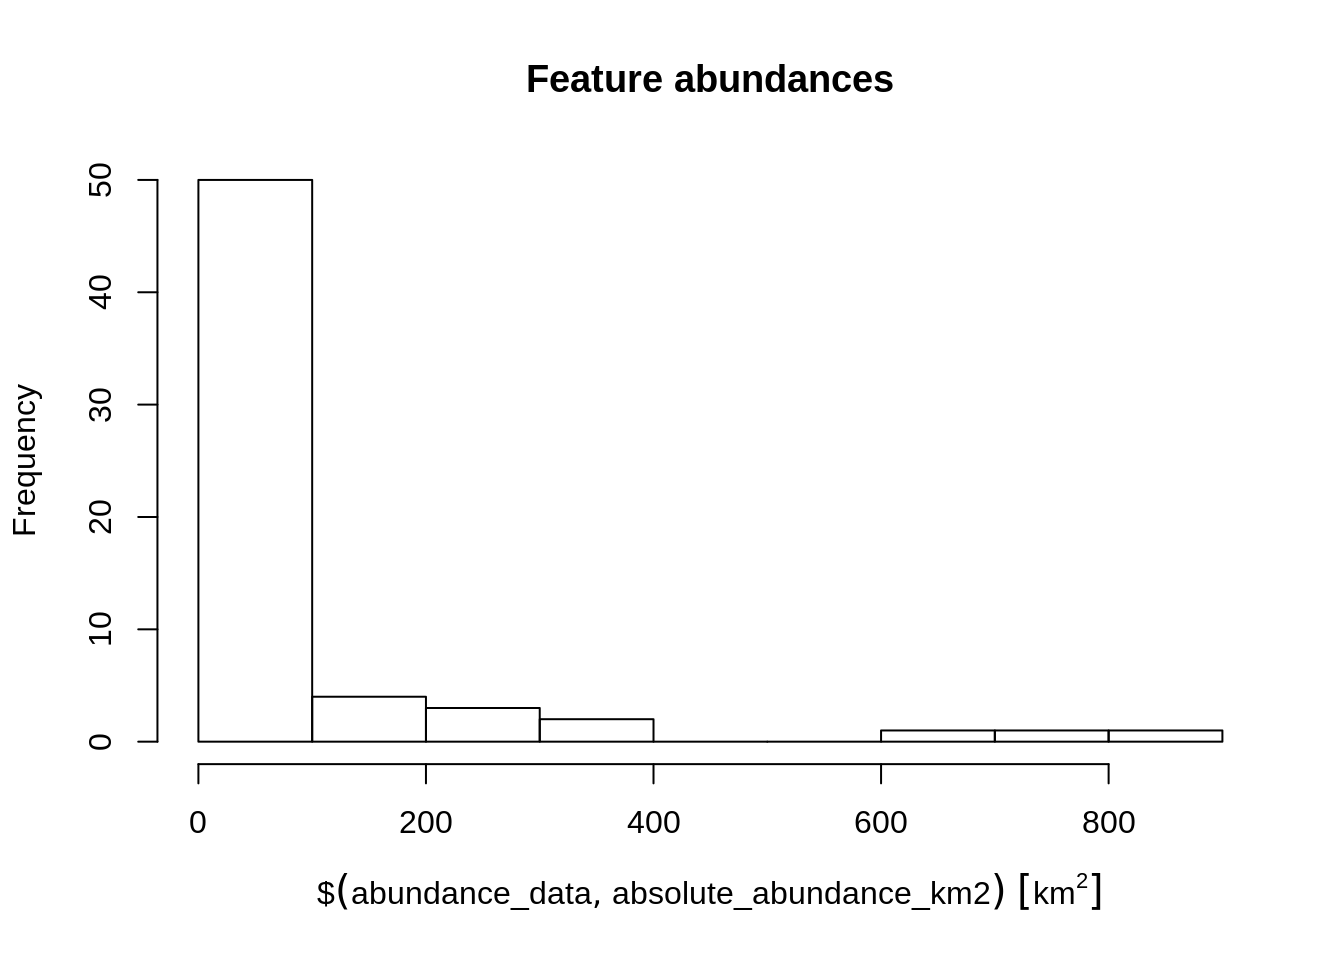
\includegraphics{prioritizr-workshop-manual_files/figure-latex/unnamed-chunk-29-1} \end{center}

\begin{Shaded}
\begin{Highlighting}[]
\CommentTok{# find the abundance of the feature with the largest abundance}
\KeywordTok{max}\NormalTok{(abundance_data}\OperatorTok{$}\NormalTok{absolute_abundance_km2)}
\end{Highlighting}
\end{Shaded}

\begin{verbatim}
## 895 [km^2]
\end{verbatim}

\begin{Shaded}
\begin{Highlighting}[]
\CommentTok{# find the name of the feature with the largest abundance}
\NormalTok{abundance_data}\OperatorTok{$}\NormalTok{feature[}\KeywordTok{which.max}\NormalTok{(abundance_data}\OperatorTok{$}\NormalTok{absolute_abundance_km2)]}
\end{Highlighting}
\end{Shaded}

\begin{verbatim}
## [1] "vegetation.20"
\end{verbatim}

Now, try to answer the following questions.

\BeginKnitrBlock{rmdquestion}
\begin{enumerate}
\def\labelenumi{\arabic{enumi}.}
\tightlist
\item
  What is the median abundance of the features (hint: \texttt{median})?
\item
  What is the abundance of the feature with smallest abundance?
\item
  What is the name of the feature with smallest abundance?
\item
  What is the total abundance of all features in the planning units
  summed together?
\item
  How many features have a total abundance greater than 100 km\^{}2
  (hint:
  \texttt{sum(abundance\_values\ \textgreater{}\ set\_units(threshold\_value,\ km\^{}2)})?
\end{enumerate}
\EndKnitrBlock{rmdquestion}

\section{Feature representation by protected
areas}\label{feature-representation-by-protected-areas}

After calculating the total amount of each feature in the planning units
(i.e.~the features' abundances), we will now calculate the amount of
each feature in the planning units that are covered by protected areas
(i.e.~feature representation by protected areas). We can complete this
task using the \texttt{feature\_representation} function. This function
requires (i) a conservation problem object with the planning unit and
biodiversity data and also (ii) an object representing a solution to the
problem (i.e an object in the same format as the planning unit data with
zeros and ones indicating if the planning units are contained in the
prioritization problem or not).

\begin{Shaded}
\begin{Highlighting}[]
\CommentTok{# create column in planning unit data with binary values (zeros and ones)}
\CommentTok{# indicating if a planning unit is covered by protected areas or not}
\NormalTok{pu_data}\OperatorTok{$}\NormalTok{pa_status <-}\StringTok{ }\KeywordTok{as.numeric}\NormalTok{(pu_data}\OperatorTok{$}\NormalTok{locked_in)}

\CommentTok{# calculate feature representation by protected areas}
\NormalTok{repr_data <-}\StringTok{ }\KeywordTok{feature_representation}\NormalTok{(p0, pu_data[, }\StringTok{"pa_status"}\NormalTok{])}

\CommentTok{# print feature representation data}
\KeywordTok{print}\NormalTok{(repr_data)}
\end{Highlighting}
\end{Shaded}

\begin{verbatim}
## # A tibble: 62 x 3
##    feature       absolute_held relative_held
##    <chr>                 <dbl>         <dbl>
##  1 vegetation.1              1        0.0303
##  2 vegetation.2             14        0.0809
##  3 vegetation.3              2        0.0833
##  4 vegetation.4              1        0.0323
##  5 vegetation.5              0        0     
##  6 vegetation.6              0        0     
##  7 vegetation.7              0        0     
##  8 vegetation.8              6        0.133 
##  9 vegetation.9             20        0.0521
## 10 vegetation.10             0        0     
## # ... with 52 more rows
\end{verbatim}

Similar to the abundance data before, the \texttt{repr\_data} object
contains three columns. The \texttt{feature} column contains the name of
each feature, the \texttt{absolute\_held} column shows the total amount
of each feature held in the solution (i.e.~the planning units covered by
protected areas), and the \texttt{relative\_held} column shows the
proportion of each feature held in the solution (i.e.~the proportion of
each feature's spatial distribution held in protected areas). Since the
\texttt{absolute\_held} values correspond to the number of grid cells in
the \texttt{veg\_data} object with overlap with protected areas, let's
convert them to aerial-based units (i.e.~km\textsuperscript{2}) so we
can report them.

\begin{Shaded}
\begin{Highlighting}[]
\CommentTok{# add new column with the areas represented in km^2}
\NormalTok{repr_data}\OperatorTok{$}\NormalTok{absolute_held_km2 <-}
\StringTok{  }\NormalTok{(repr_data}\OperatorTok{$}\NormalTok{absolute_held }\OperatorTok{*}\StringTok{ }\KeywordTok{prod}\NormalTok{(}\KeywordTok{res}\NormalTok{(veg_data))) }\OperatorTok
\StringTok{  }\KeywordTok{set_units}\NormalTok{(m}\OperatorTok{^}\DecValTok{2}\NormalTok{) }\OperatorTok
\StringTok{  }\KeywordTok{set_units}\NormalTok{(km}\OperatorTok{^}\DecValTok{2}\NormalTok{)}

\CommentTok{# print representation data}
\KeywordTok{print}\NormalTok{(repr_data)}
\end{Highlighting}
\end{Shaded}

\begin{verbatim}
## # A tibble: 62 x 4
##    feature       absolute_held relative_held absolute_held_km2
##    <chr>                 <dbl>         <dbl>            [km^2]
##  1 vegetation.1              1        0.0303                 1
##  2 vegetation.2             14        0.0809                14
##  3 vegetation.3              2        0.0833                 2
##  4 vegetation.4              1        0.0323                 1
##  5 vegetation.5              0        0                      0
##  6 vegetation.6              0        0                      0
##  7 vegetation.7              0        0                      0
##  8 vegetation.8              6        0.133                  6
##  9 vegetation.9             20        0.0521                20
## 10 vegetation.10             0        0                      0
## # ... with 52 more rows
\end{verbatim}

Now let's investigate how well the species are represented.

\BeginKnitrBlock{rmdquestion}
\begin{enumerate}
\def\labelenumi{\arabic{enumi}.}
\tightlist
\item
  What is the average proportion of the features held in protected areas
  (hint: \texttt{mean(x,\ na.rm\ =\ TRUE)}?
\item
  What is the average amount of land in km\textsuperscript{2} that
  features are represented by protected areas?
\item
  What is the name of the feature with the greatest proportionate
  coverage by protected areas?
\item
  What is the name of the feature with the greatest aerial coverage by
  protected areas?
\item
  Do questions two and three have the same answer? If not, why could
  this be?
\item
  Is there a relationship between the total abundance of a feature and
  how well it is represented by protected areas (hint:
  \texttt{plot(abundances\ \textasciitilde{}\ relative\_held)})?
\item
  Are any features entirely missing from protected areas (hint:
  \texttt{sum(x\ ==\ 0)})?
\item
  If we set a target of 10\% coverage by protected areas, how many
  features fail to meet this target (hint:
  \texttt{sum(relative\_held\ \textgreater{}=\ target)})?
\item
  If we set a target of 20\% coverage by protected areas, how many
  features fail to meet this target?
\end{enumerate}
\EndKnitrBlock{rmdquestion}

\chapter{Spatial prioritizations}\label{spatial-prioritizations}

\section{Introduction}\label{introduction-2}

Here we will develop prioritizations to identify priority areas for
protected area establishment. Its worth noting that
\href{https://prioritizr.net/}{prioritizr},
\href{http://marxan.org/}{Marxan}, and
\href{https://www.helsinki.fi/en/researchgroups/digital-geography-lab/software-developed-in-cbig\#section-52992}{Zonation}
are all decision \emph{support} tools. This means that these tools are
all designed to \emph{help} you make decisions---they can't make
decisions for you.

\section{Starting out simple}\label{starting-out-simple}

To start things off, let's keep things simple. Let's create a
prioritization using the
\href{https://prioritizr.net/reference/add_min_set_objective.html}{minimum
set problem formulation of the reserve selection problem}. This problem
will have 5\% targets for each vegetation class and use the data in the
\texttt{cost} column to specify acquisition costs. Although we strongly
recommend using \href{https://www.gurobi.com/}{Gurobi} to solve problems
(with
\href{https://prioritizr.net/reference/add_gurobi_solver.html}{\texttt{add\_gurobi\_solver}}),
we will use the
\href{https://prioritizr.net/reference/add_lsymphony_solver.html}{lpsymphony
solver} in this workshop since it is much easier to install. The Gurobi
solver is the fastest solver that prioritizr can use to generate
solutions and it is much, much, much faster than the lpsymphony solver
(\href{https://prioritizr.net/articles/gurobi_installation.html}{see
here for Gurobi installation instructions}).

\begin{Shaded}
\begin{Highlighting}[]
\CommentTok{# print planning unit data}
\KeywordTok{print}\NormalTok{(pu_data)}
\end{Highlighting}
\end{Shaded}

\begin{verbatim}
## class       : SpatialPolygonsDataFrame 
## features    : 1130 
## extent      : 1080623, 1399989, -4840595, -4497092  (xmin, xmax, ymin, ymax)
## crs         : +proj=aea +lat_1=-18 +lat_2=-36 +lat_0=0 +lon_0=132 +x_0=0 +y_0=0 +ellps=GRS80 +units=m +no_defs 
## variables   : 6
## names       :   id,              cost, status, locked_in, locked_out, pa_status 
## min values  :    1, 0.192488262910798,      0,         0,          0,         0 
## max values  : 1130,  61.9272727272727,      2,         1,          1,         1
\end{verbatim}

\begin{Shaded}
\begin{Highlighting}[]
\CommentTok{# make prioritization problem}
\NormalTok{p1 <-}\StringTok{ }\KeywordTok{problem}\NormalTok{(pu_data, veg_data, }\DataTypeTok{cost_column =} \StringTok{"cost"}\NormalTok{) }\OperatorTok
\StringTok{      }\KeywordTok{add_min_set_objective}\NormalTok{() }\OperatorTok
\StringTok{      }\KeywordTok{add_relative_targets}\NormalTok{(}\FloatTok{0.05}\NormalTok{) }\OperatorTok\StringTok{ }\CommentTok{# 5% representation targets}
\StringTok{      }\KeywordTok{add_binary_decisions}\NormalTok{() }\OperatorTok
\StringTok{      }\KeywordTok{add_lpsymphony_solver}\NormalTok{(}\DataTypeTok{verbose =} \OtherTok{FALSE}\NormalTok{)}

\CommentTok{# print problem}
\KeywordTok{print}\NormalTok{(p1)}
\end{Highlighting}
\end{Shaded}

\begin{verbatim}
## Conservation Problem
##   planning units: SpatialPolygonsDataFrame (1130 units)
##   cost:           min: 0.19249, max: 61.92727
##   features:       vegetation.1, vegetation.2, vegetation.3, ... (62 features)
##   objective:      Minimum set objective 
##   targets:        Relative targets [targets (min: 0.05, max: 0.05)]
##   decisions:      Binary decision 
##   constraints:    <none>
##   penalties:      <none>
##   portfolio:      default
##   solver:         Lpsymphony [first_feasible (0), gap (0.1), time_limit (-1), verbose (0)]
\end{verbatim}

\begin{Shaded}
\begin{Highlighting}[]
\CommentTok{# solve problem}
\NormalTok{s1 <-}\StringTok{ }\KeywordTok{solve}\NormalTok{(p1)}

\CommentTok{# print solution,}
\CommentTok{# the solution_1 column contains the solution values with binary values}
\CommentTok{# indicating if a planning unit was selected as a (1) priority area or (0) not}
\KeywordTok{print}\NormalTok{(s1)}
\end{Highlighting}
\end{Shaded}

\begin{verbatim}
## class       : SpatialPolygonsDataFrame 
## features    : 1130 
## extent      : 1080623, 1399989, -4840595, -4497092  (xmin, xmax, ymin, ymax)
## crs         : +proj=aea +lat_1=-18 +lat_2=-36 +lat_0=0 +lon_0=132 +x_0=0 +y_0=0 +ellps=GRS80 +units=m +no_defs 
## variables   : 7
## names       :   id,              cost, status, locked_in, locked_out, pa_status, solution_1 
## min values  :    1, 0.192488262910798,      0,         0,          0,         0,          0 
## max values  : 1130,  61.9272727272727,      2,         1,          1,         1,          1
\end{verbatim}

\begin{Shaded}
\begin{Highlighting}[]
\CommentTok{# calculate number of planning units selected in the prioritization}
\KeywordTok{sum}\NormalTok{(s1}\OperatorTok{$}\NormalTok{solution_}\DecValTok{1}\NormalTok{)}
\end{Highlighting}
\end{Shaded}

\begin{verbatim}
## [1] 36
\end{verbatim}

\begin{Shaded}
\begin{Highlighting}[]
\CommentTok{# calculate total cost of the prioritization}
\KeywordTok{sum}\NormalTok{(s1}\OperatorTok{$}\NormalTok{solution_}\DecValTok{1} \OperatorTok{*}\StringTok{ }\NormalTok{s1}\OperatorTok{$}\NormalTok{cost)}
\end{Highlighting}
\end{Shaded}

\begin{verbatim}
## [1] 806.2393
\end{verbatim}

\begin{Shaded}
\begin{Highlighting}[]
\CommentTok{# plot solution}
\KeywordTok{spplot}\NormalTok{(s1, }\StringTok{"solution_1"}\NormalTok{, }\DataTypeTok{col.regions =} \KeywordTok{c}\NormalTok{(}\StringTok{"white"}\NormalTok{, }\StringTok{"darkgreen"}\NormalTok{), }\DataTypeTok{main =} \StringTok{"s1"}\NormalTok{)}
\end{Highlighting}
\end{Shaded}

\begin{center}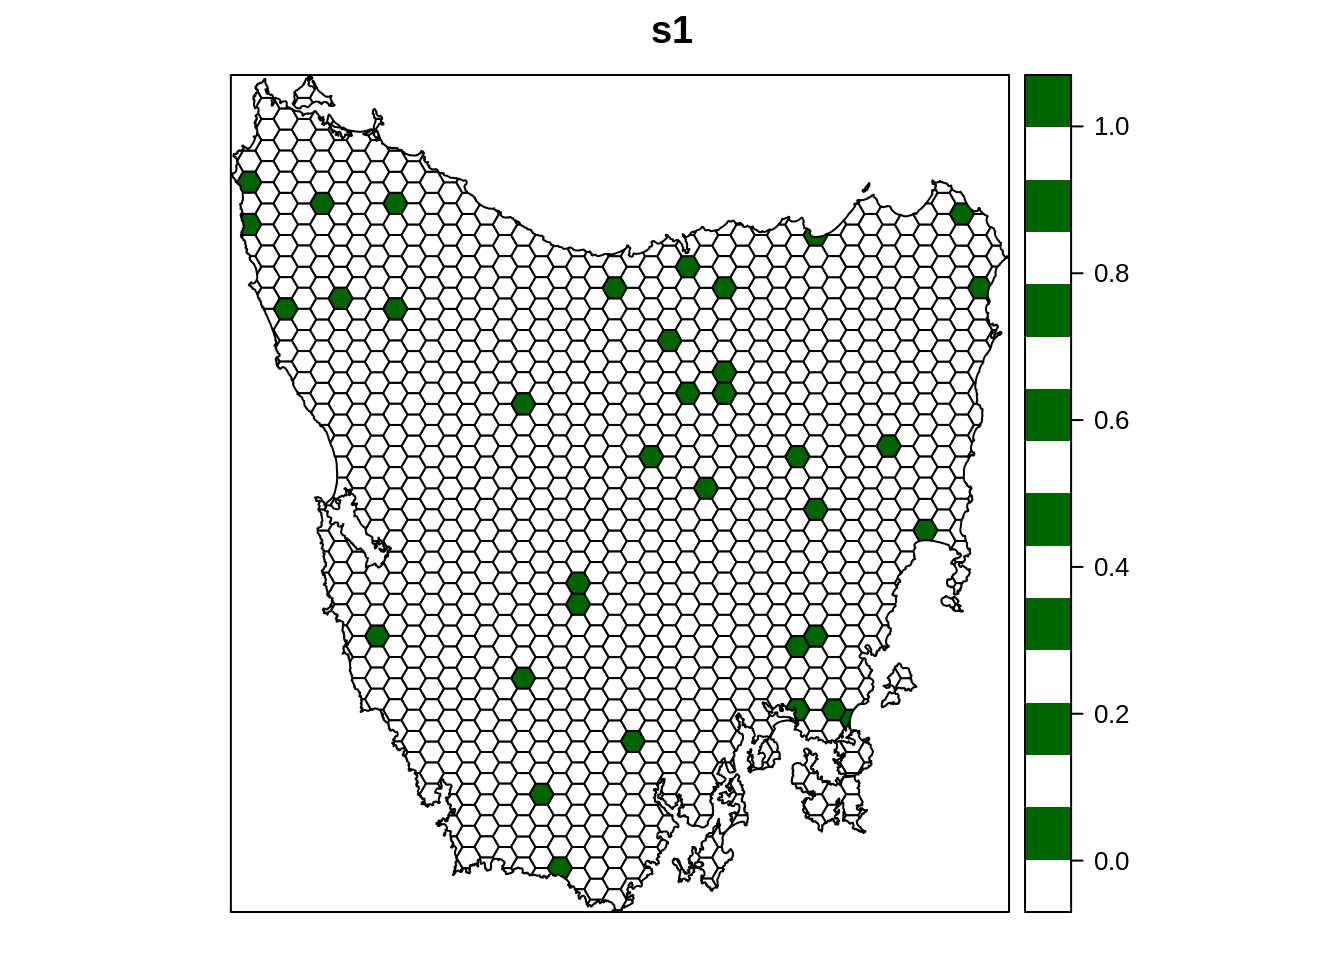
\includegraphics[width=0.65\linewidth]{prioritizr-workshop-manual_files/figure-latex/unnamed-chunk-34-1} \end{center}

Now let's examine the solution.

\BeginKnitrBlock{rmdquestion}
\begin{enumerate}
\def\labelenumi{\arabic{enumi}.}
\tightlist
\item
  How many planing units were selected in the prioritization? What
  proportion of planning units were selected in the prioritization?
\item
  Is there a pattern in the spatial distribution of the priority areas?
\item
  Can you verify that all of the targets were met in the prioritization
  (hint:
  \texttt{feature\_representation(p1,\ s1{[},\ "solution\_1"{]})})?
\item
  What are limitations of this prioritization?
\end{enumerate}
\EndKnitrBlock{rmdquestion}

\section{Adding complexity}\label{adding-complexity}

Our first prioritization suffers many limitations, so let's add
additional constraints to the problem to make it more useful. First,
let's lock in planing units that are already inside protected areas.

\begin{Shaded}
\begin{Highlighting}[]
\CommentTok{# make prioritization problem}
\NormalTok{p2 <-}\StringTok{ }\KeywordTok{problem}\NormalTok{(pu_data, veg_data, }\DataTypeTok{cost_column =} \StringTok{"cost"}\NormalTok{) }\OperatorTok
\StringTok{      }\KeywordTok{add_min_set_objective}\NormalTok{() }\OperatorTok
\StringTok{      }\KeywordTok{add_relative_targets}\NormalTok{(}\FloatTok{0.05}\NormalTok{) }\OperatorTok
\StringTok{      }\KeywordTok{add_locked_in_constraints}\NormalTok{(}\StringTok{"locked_in"}\NormalTok{) }\OperatorTok
\StringTok{      }\KeywordTok{add_binary_decisions}\NormalTok{() }\OperatorTok
\StringTok{      }\KeywordTok{add_lpsymphony_solver}\NormalTok{(}\DataTypeTok{verbose =} \OtherTok{FALSE}\NormalTok{)}

\CommentTok{# print problem}
\KeywordTok{print}\NormalTok{(p2)}
\end{Highlighting}
\end{Shaded}

\begin{verbatim}
## Conservation Problem
##   planning units: SpatialPolygonsDataFrame (1130 units)
##   cost:           min: 0.19249, max: 61.92727
##   features:       vegetation.1, vegetation.2, vegetation.3, ... (62 features)
##   objective:      Minimum set objective 
##   targets:        Relative targets [targets (min: 0.05, max: 0.05)]
##   decisions:      Binary decision 
##   constraints:    <Locked in planning units [257 locked units]>
##   penalties:      <none>
##   portfolio:      default
##   solver:         Lpsymphony [first_feasible (0), gap (0.1), time_limit (-1), verbose (0)]
\end{verbatim}

\begin{Shaded}
\begin{Highlighting}[]
\CommentTok{# solve problem}
\NormalTok{s2 <-}\StringTok{ }\KeywordTok{solve}\NormalTok{(p2)}

\CommentTok{# plot solution}
\KeywordTok{spplot}\NormalTok{(s2, }\StringTok{"solution_1"}\NormalTok{, }\DataTypeTok{col.regions =} \KeywordTok{c}\NormalTok{(}\StringTok{"white"}\NormalTok{, }\StringTok{"darkgreen"}\NormalTok{), }\DataTypeTok{main =} \StringTok{"s2"}\NormalTok{)}
\end{Highlighting}
\end{Shaded}

\begin{center}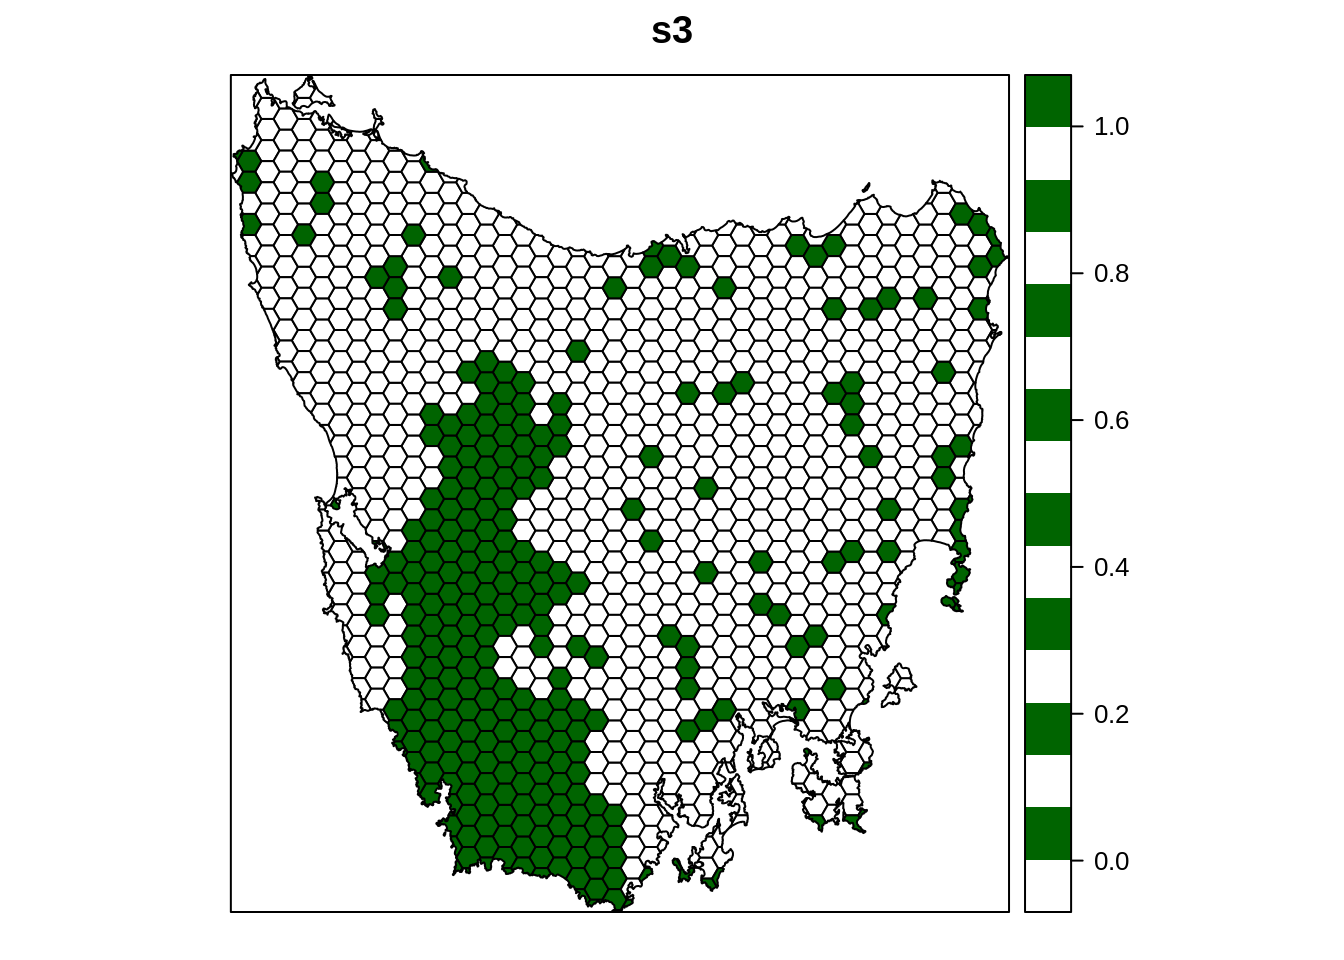
\includegraphics[width=0.65\linewidth]{prioritizr-workshop-manual_files/figure-latex/unnamed-chunk-36-1} \end{center}

Let's pretend we talked to an expert on the vegetation communities in
our study system and they recommended that a 20\% target was needed. So,
now let's set the targets to 20\% of their total distribution in the
study area.

\begin{Shaded}
\begin{Highlighting}[]
\CommentTok{# make prioritization problem}
\NormalTok{p3 <-}\StringTok{ }\KeywordTok{problem}\NormalTok{(pu_data, veg_data, }\DataTypeTok{cost_column =} \StringTok{"cost"}\NormalTok{) }\OperatorTok
\StringTok{      }\KeywordTok{add_min_set_objective}\NormalTok{() }\OperatorTok
\StringTok{      }\KeywordTok{add_relative_targets}\NormalTok{(}\FloatTok{0.2}\NormalTok{) }\OperatorTok
\StringTok{      }\KeywordTok{add_locked_in_constraints}\NormalTok{(}\StringTok{"locked_in"}\NormalTok{) }\OperatorTok
\StringTok{      }\KeywordTok{add_binary_decisions}\NormalTok{() }\OperatorTok
\StringTok{      }\KeywordTok{add_lpsymphony_solver}\NormalTok{(}\DataTypeTok{verbose =} \OtherTok{FALSE}\NormalTok{)}

\CommentTok{# print problem}
\KeywordTok{print}\NormalTok{(p3)}
\end{Highlighting}
\end{Shaded}

\begin{verbatim}
## Conservation Problem
##   planning units: SpatialPolygonsDataFrame (1130 units)
##   cost:           min: 0.19249, max: 61.92727
##   features:       vegetation.1, vegetation.2, vegetation.3, ... (62 features)
##   objective:      Minimum set objective 
##   targets:        Relative targets [targets (min: 0.2, max: 0.2)]
##   decisions:      Binary decision 
##   constraints:    <Locked in planning units [257 locked units]>
##   penalties:      <none>
##   portfolio:      default
##   solver:         Lpsymphony [first_feasible (0), gap (0.1), time_limit (-1), verbose (0)]
\end{verbatim}

\begin{Shaded}
\begin{Highlighting}[]
\CommentTok{# solve problem}
\NormalTok{s3 <-}\StringTok{ }\KeywordTok{solve}\NormalTok{(p3)}

\CommentTok{# plot solution}
\KeywordTok{spplot}\NormalTok{(s3, }\StringTok{"solution_1"}\NormalTok{, }\DataTypeTok{col.regions =} \KeywordTok{c}\NormalTok{(}\StringTok{"white"}\NormalTok{, }\StringTok{"darkgreen"}\NormalTok{), }\DataTypeTok{main =} \StringTok{"s3"}\NormalTok{)}
\end{Highlighting}
\end{Shaded}

\begin{center}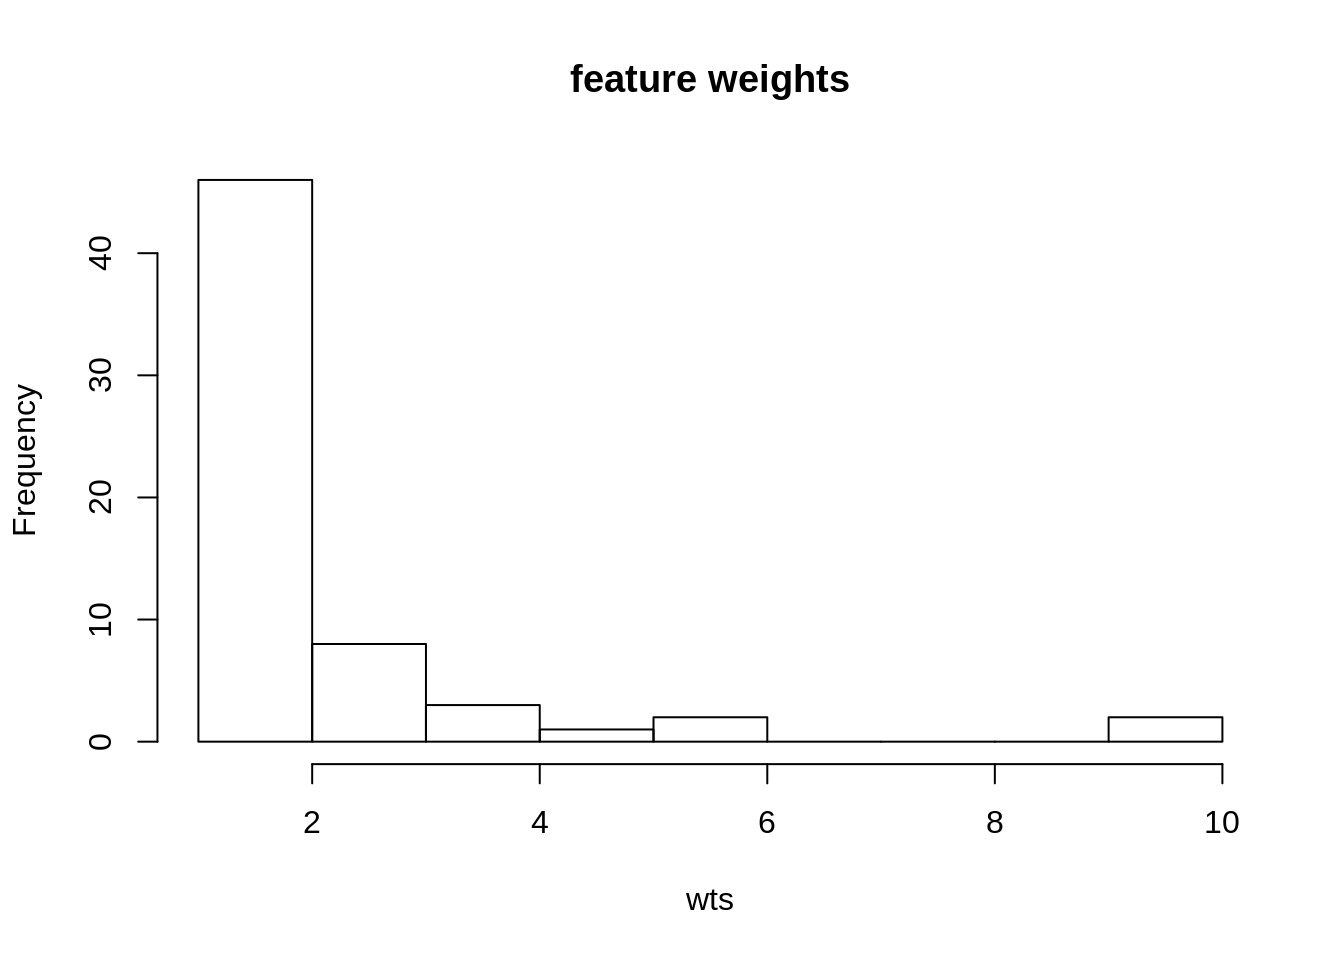
\includegraphics[width=0.65\linewidth]{prioritizr-workshop-manual_files/figure-latex/unnamed-chunk-37-1} \end{center}

Next, let's lock out highly degraded areas.

\begin{Shaded}
\begin{Highlighting}[]
\CommentTok{# make prioritization problem}
\NormalTok{p4 <-}\StringTok{ }\KeywordTok{problem}\NormalTok{(pu_data, veg_data, }\DataTypeTok{cost_column =} \StringTok{"cost"}\NormalTok{) }\OperatorTok
\StringTok{      }\KeywordTok{add_min_set_objective}\NormalTok{() }\OperatorTok
\StringTok{      }\KeywordTok{add_relative_targets}\NormalTok{(}\FloatTok{0.2}\NormalTok{) }\OperatorTok
\StringTok{      }\KeywordTok{add_locked_in_constraints}\NormalTok{(}\StringTok{"locked_in"}\NormalTok{) }\OperatorTok
\StringTok{      }\KeywordTok{add_locked_out_constraints}\NormalTok{(}\StringTok{"locked_out"}\NormalTok{) }\OperatorTok
\StringTok{      }\KeywordTok{add_binary_decisions}\NormalTok{() }\OperatorTok
\StringTok{      }\KeywordTok{add_lpsymphony_solver}\NormalTok{(}\DataTypeTok{verbose =} \OtherTok{FALSE}\NormalTok{)}
\end{Highlighting}
\end{Shaded}

\begin{Shaded}
\begin{Highlighting}[]
\CommentTok{# print problem}
\KeywordTok{print}\NormalTok{(p4)}
\end{Highlighting}
\end{Shaded}

\begin{verbatim}
## Conservation Problem
##   planning units: SpatialPolygonsDataFrame (1130 units)
##   cost:           min: 0.19249, max: 61.92727
##   features:       vegetation.1, vegetation.2, vegetation.3, ... (62 features)
##   objective:      Minimum set objective 
##   targets:        Relative targets [targets (min: 0.2, max: 0.2)]
##   decisions:      Binary decision 
##   constraints:    <Locked out planning units [51 locked units]
##                    Locked in planning units [257 locked units]>
##   penalties:      <none>
##   portfolio:      default
##   solver:         Lpsymphony [first_feasible (0), gap (0.1), time_limit (-1), verbose (0)]
\end{verbatim}

\begin{Shaded}
\begin{Highlighting}[]
\CommentTok{# solve problem}
\NormalTok{s4 <-}\StringTok{ }\KeywordTok{solve}\NormalTok{(p4)}

\CommentTok{# plot solution}
\KeywordTok{spplot}\NormalTok{(s4, }\StringTok{"solution_1"}\NormalTok{, }\DataTypeTok{col.regions =} \KeywordTok{c}\NormalTok{(}\StringTok{"white"}\NormalTok{, }\StringTok{"darkgreen"}\NormalTok{), }\DataTypeTok{main =} \StringTok{"s4"}\NormalTok{)}
\end{Highlighting}
\end{Shaded}

\begin{center}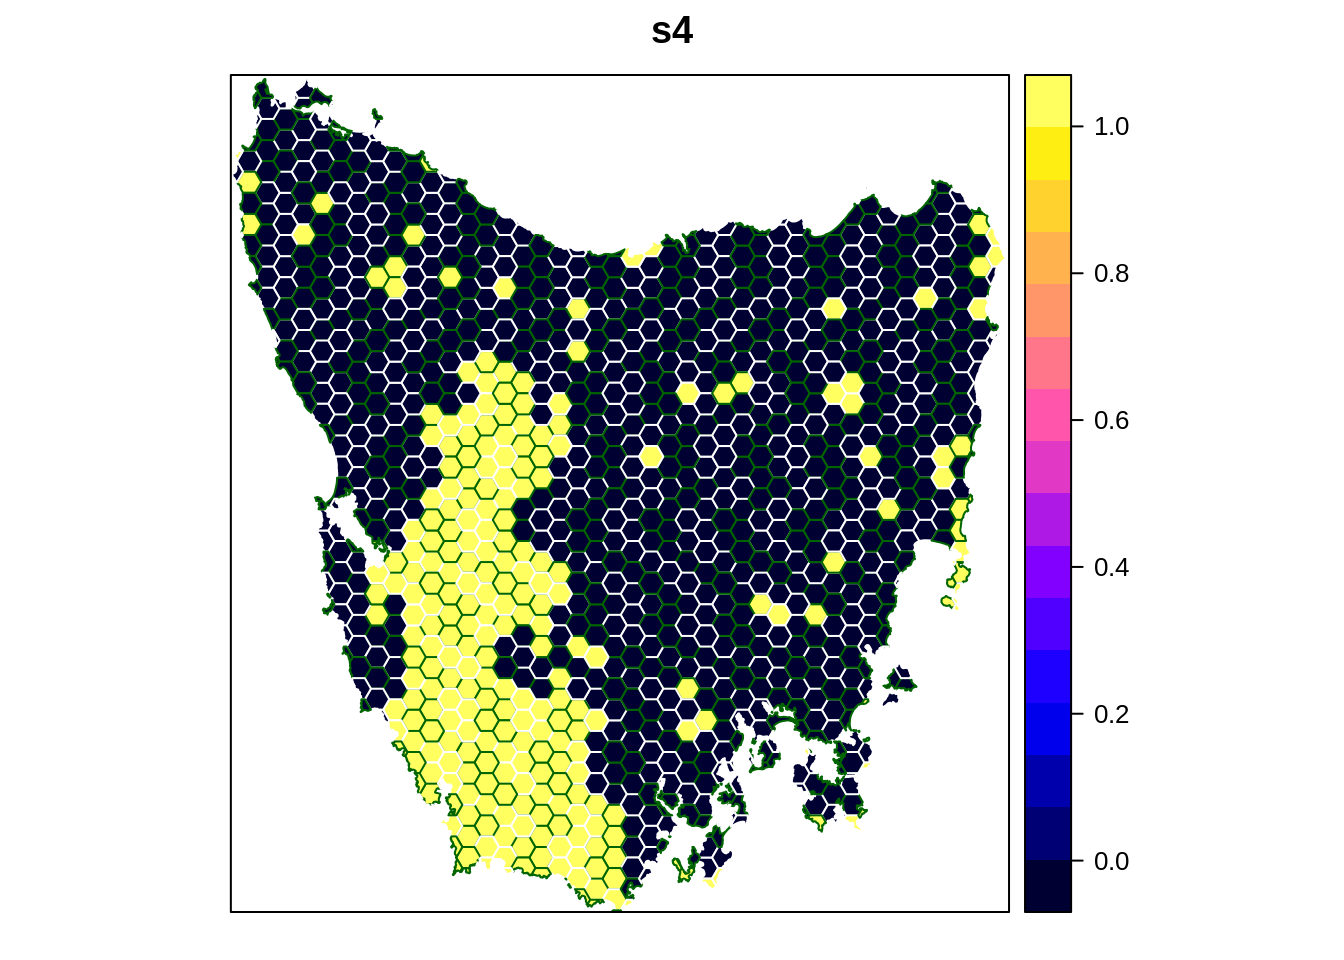
\includegraphics[width=0.65\linewidth]{prioritizr-workshop-manual_files/figure-latex/unnamed-chunk-39-1} \end{center}

\clearpage

Now, let's compare the solutions.

\BeginKnitrBlock{rmdquestion}
\begin{enumerate}
\def\labelenumi{\arabic{enumi}.}
\tightlist
\item
  What is the cost of the planning units selected in \texttt{s2},
  \texttt{s3}, and \texttt{s4}?
\item
  How many planning units are in \texttt{s2}, \texttt{s3}, and
  \texttt{s4}?
\item
  Do the solutions with more planning units have a greater cost? Why or
  why not?
\item
  Why does the first solution (\texttt{s1}) cost less than the second
  solution with protected areas locked into the solution (\texttt{s2})?
\item
  Why does the third solution (\texttt{s3}) cost less than the fourth
  solution solution with highly degraded areas locked out (\texttt{s4})?
\item
  Since planning units covered by existing protected areas have already
  been purchased, what is the cost for expanding the protected area
  system based on on the fourth prioritization (\texttt{s4}) (hint:
  total cost minus the cost of locked in planning units)?
\item
  What happens if you specify targets that exceed the total amount of
  vegetation in the study area and try to solve the problem? You can do
  this by modifying the code to make \texttt{p4} with
  \texttt{add\_absolute\_targets(1000)} instead of
  \texttt{add\_relative\_targets(0.2)} and generating a new solution.
\end{enumerate}
\EndKnitrBlock{rmdquestion}

\section{Penalizing fragmentation}\label{penalizing-fragmentation}

Plans for protected area systems should facilitate gene flow and
dispersal between individual reserves in the system. However, the
prioritizations we have made so far have been highly fragmented. Similar
to the Marxan decision support tool, we can add penalties to our
conservation planning problem to penalize fragmentation (i.e.~total
exposed boundary length) and we also need to set a useful penalty value
when adding such penalties (akin to Marxan's boundary length multiplier
value; BLM). If we set our penalty value too low, then we end up with a
solution that is identical to the solution with no added penalties. If
we set our penalty value too high, then prioritizr will take a long time
to solve the problem and we will end up with a solution that contains
lots of extra planning units that are not needed (since the penalty
value is so high that minimizing fragmentation is more important than
cost). As a rule of thumb, we generally want penalty values between
0.00001 and 0.01 but finding a useful penalty value requires
calibration. The ``correct'' penalty value depends on the size of the
planning units, the main objective values (e.g.~cost values), and the
effect of fragmentation on biodiversity persistence. Let's create a new
problem that is similar to our previous problem (\texttt{p4}) -- except
that it contains boundary length penalties and a slightly higher
optimality gap to reduce runtime (default is 0.1) -- and solve it.

\clearpage

\begin{Shaded}
\begin{Highlighting}[]
\CommentTok{# make prioritization problem}
\NormalTok{p5 <-}\StringTok{ }\KeywordTok{problem}\NormalTok{(pu_data, veg_data, }\DataTypeTok{cost_column =} \StringTok{"cost"}\NormalTok{) }\OperatorTok
\StringTok{      }\KeywordTok{add_min_set_objective}\NormalTok{() }\OperatorTok
\StringTok{      }\KeywordTok{add_boundary_penalties}\NormalTok{(}\DataTypeTok{penalty =} \FloatTok{0.0005}\NormalTok{) }\OperatorTok
\StringTok{      }\KeywordTok{add_relative_targets}\NormalTok{(}\FloatTok{0.2}\NormalTok{) }\OperatorTok
\StringTok{      }\KeywordTok{add_locked_in_constraints}\NormalTok{(}\StringTok{"locked_in"}\NormalTok{) }\OperatorTok
\StringTok{      }\KeywordTok{add_locked_out_constraints}\NormalTok{(}\StringTok{"locked_out"}\NormalTok{) }\OperatorTok
\StringTok{      }\KeywordTok{add_binary_decisions}\NormalTok{() }\OperatorTok
\StringTok{      }\KeywordTok{add_lpsymphony_solver}\NormalTok{(}\DataTypeTok{verbose =} \OtherTok{FALSE}\NormalTok{, }\DataTypeTok{gap =} \DecValTok{1}\NormalTok{)}

\CommentTok{# print problem}
\KeywordTok{print}\NormalTok{(p5)}
\end{Highlighting}
\end{Shaded}

\begin{verbatim}
## Conservation Problem
##   planning units: SpatialPolygonsDataFrame (1130 units)
##   cost:           min: 0.19249, max: 61.92727
##   features:       vegetation.1, vegetation.2, vegetation.3, ... (62 features)
##   objective:      Minimum set objective 
##   targets:        Relative targets [targets (min: 0.2, max: 0.2)]
##   decisions:      Binary decision 
##   constraints:    <Locked in planning units [257 locked units]
##                    Locked out planning units [51 locked units]>
##   penalties:      <Boundary penalties [edge factor (min: 0.5, max: 0.5), penalty (5e-04), zones]>
##   portfolio:      default
##   solver:         Lpsymphony [first_feasible (0), gap (1), time_limit (-1), verbose (0)]
\end{verbatim}

\begin{Shaded}
\begin{Highlighting}[]
\CommentTok{# solve problem,}
\CommentTok{# note this will take around 30 seconds}
\NormalTok{s5 <-}\StringTok{ }\KeywordTok{solve}\NormalTok{(p5)}

\CommentTok{# print solution}
\KeywordTok{print}\NormalTok{(s5)}
\end{Highlighting}
\end{Shaded}

\begin{verbatim}
## class       : SpatialPolygonsDataFrame 
## features    : 1130 
## extent      : 1080623, 1399989, -4840595, -4497092  (xmin, xmax, ymin, ymax)
## crs         : +proj=aea +lat_1=-18 +lat_2=-36 +lat_0=0 +lon_0=132 +x_0=0 +y_0=0 +ellps=GRS80 +units=m +no_defs 
## variables   : 7
## names       :   id,              cost, status, locked_in, locked_out, pa_status, solution_1 
## min values  :    1, 0.192488262910798,      0,         0,          0,         0,          0 
## max values  : 1130,  61.9272727272727,      2,         1,          1,         1,          1
\end{verbatim}

\begin{Shaded}
\begin{Highlighting}[]
\CommentTok{# plot solution}
\KeywordTok{spplot}\NormalTok{(s5, }\StringTok{"solution_1"}\NormalTok{, }\DataTypeTok{col.regions =} \KeywordTok{c}\NormalTok{(}\StringTok{"white"}\NormalTok{, }\StringTok{"darkgreen"}\NormalTok{), }\DataTypeTok{main =} \StringTok{"s5"}\NormalTok{)}
\end{Highlighting}
\end{Shaded}

\begin{center}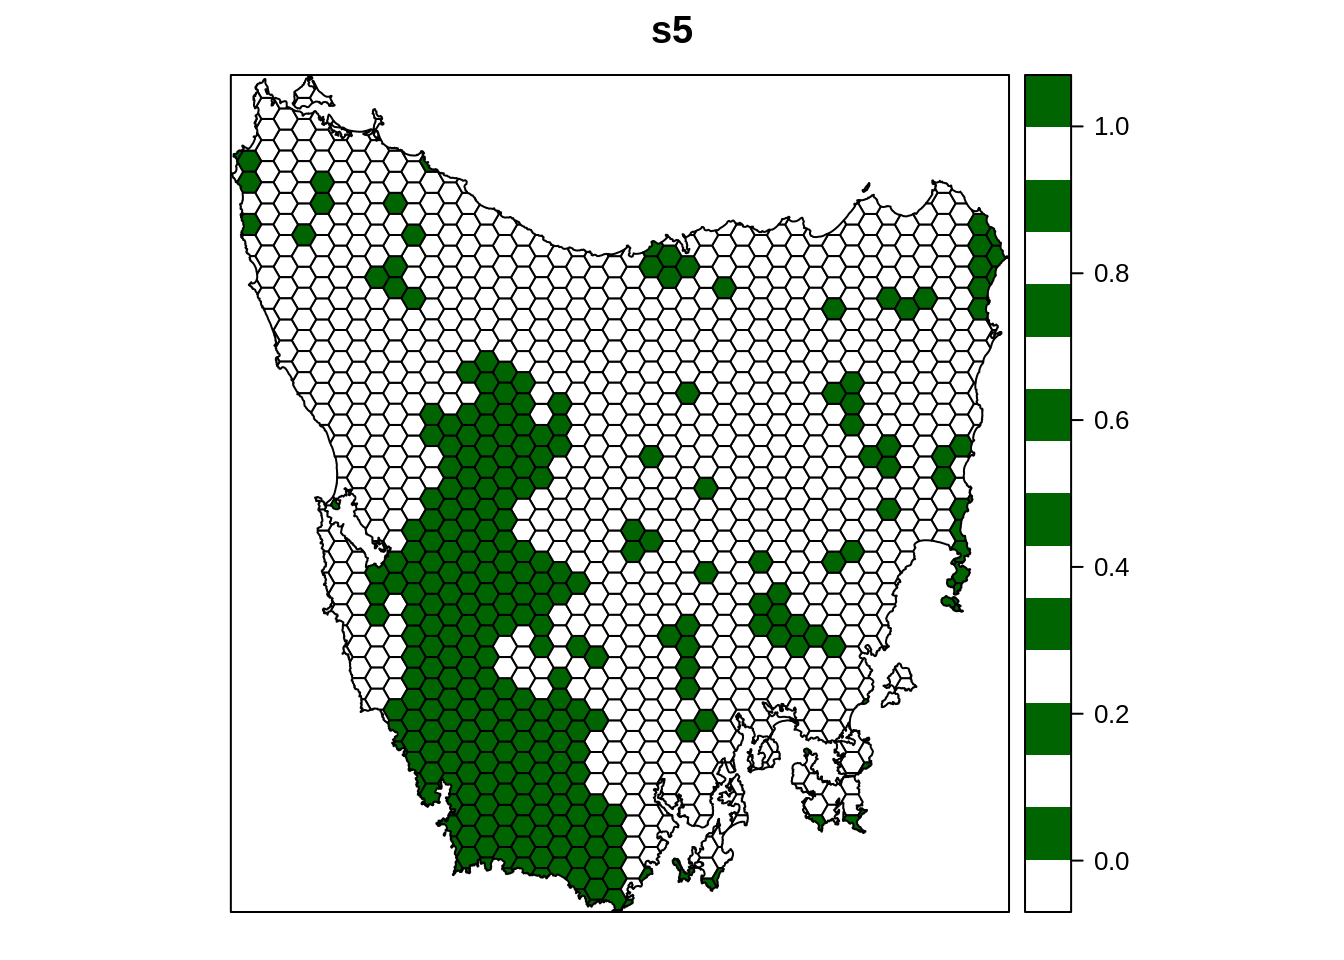
\includegraphics[width=0.65\linewidth]{prioritizr-workshop-manual_files/figure-latex/unnamed-chunk-41-1} \end{center}

Now let's compare the solutions to the problems with (\texttt{s5}) and
without (\texttt{s4}) the boundary length penalties.

\BeginKnitrBlock{rmdquestion}
\begin{enumerate}
\def\labelenumi{\arabic{enumi}.}
\tightlist
\item
  What is the cost the fourth (\texttt{s4}) and fifth (\texttt{s5})
  solutions? Why does the fifth solution (\texttt{s5}) cost more than
  the fourth (\texttt{s4}) solution?
\item
  Try setting the penalty value to 0.000000001 (i.e. \texttt{1e-9})
  instead of 0.001. What is the cost of the solution now? Is it
  different from the fourth solution (\texttt{s4}) (hint: try plotting
  the solutions to visualize them)? Is this is a useful penalty value?
  Why?
\item
  Try setting the penalty value to 0.5. What is the cost of the solution
  now? Is it different from the fourth solution (\texttt{s4}) (hint: try
  plotting the solutions to visualize them)? Is this a useful penalty
  value? Why?
\end{enumerate}
\EndKnitrBlock{rmdquestion}

\clearpage

\section{Budget limited
prioritizations}\label{budget-limited-prioritizations}

In the real-world, the funding available for conservation is often very
limited. As a consequence, decision makers often need prioritizations
where the total cost of priority areas does not exceed a budget. In our
fourth prioritization (\texttt{s4}), we found that we would need to
spend an additional \$909 million AUD to ensure that each vegetation
community is adequately represented in the protected area system. But
what if the funds available for protecting new land were limited to
\$100 million AUD? In this case, we need a ``budget limited
prioritization''. Budget limited prioritizations aim to maximize some
measure of conservation benefit subject to a budget (e.g.
\href{https://prioritizr.net/reference/add_max_cover_objective.html}{number
of species with at least one occurrence in the protected area system},
or
\href{https://prioritizr.net/reference/add_max_phylo_div_objective.html}{phylogenetic
diversity}). Let's create a budget limited prioritization that aims to
adequately represent as many targets as possible whilst remaining within
a budget.

\begin{Shaded}
\begin{Highlighting}[]
\CommentTok{# set the funds for additional land acquisition}
\NormalTok{funds <-}\StringTok{ }\DecValTok{100}

\CommentTok{# calculate the total budget for the prioritization}
\NormalTok{budget <-}\StringTok{ }\NormalTok{funds }\OperatorTok{+}\StringTok{ }\KeywordTok{sum}\NormalTok{(s4}\OperatorTok{$}\NormalTok{cost }\OperatorTok{*}\StringTok{ }\NormalTok{s4}\OperatorTok{$}\NormalTok{locked_in)}
\KeywordTok{print}\NormalTok{(budget)}
\end{Highlighting}
\end{Shaded}

\begin{verbatim}
## [1] 8575.56
\end{verbatim}

\begin{Shaded}
\begin{Highlighting}[]
\CommentTok{# make prioritization problem}
\NormalTok{p6 <-}\StringTok{ }\KeywordTok{problem}\NormalTok{(pu_data, veg_data, }\DataTypeTok{cost_column =} \StringTok{"cost"}\NormalTok{) }\OperatorTok
\StringTok{      }\KeywordTok{add_max_features_objective}\NormalTok{(budget) }\OperatorTok
\StringTok{      }\KeywordTok{add_relative_targets}\NormalTok{(}\FloatTok{0.2}\NormalTok{) }\OperatorTok
\StringTok{      }\KeywordTok{add_locked_in_constraints}\NormalTok{(}\StringTok{"locked_in"}\NormalTok{) }\OperatorTok
\StringTok{      }\KeywordTok{add_locked_out_constraints}\NormalTok{(}\StringTok{"locked_out"}\NormalTok{) }\OperatorTok
\StringTok{      }\KeywordTok{add_binary_decisions}\NormalTok{() }\OperatorTok
\StringTok{      }\KeywordTok{add_lpsymphony_solver}\NormalTok{(}\DataTypeTok{verbose =} \OtherTok{FALSE}\NormalTok{)}

\CommentTok{# print problem}
\KeywordTok{print}\NormalTok{(p6)}
\end{Highlighting}
\end{Shaded}

\begin{verbatim}
## Conservation Problem
##   planning units: SpatialPolygonsDataFrame (1130 units)
##   cost:           min: 0.19249, max: 61.92727
##   features:       vegetation.1, vegetation.2, vegetation.3, ... (62 features)
##   objective:      Maximum representation objective [budget (8575.56009869836)]
##   targets:        Relative targets [targets (min: 0.2, max: 0.2)]
##   decisions:      Binary decision 
##   constraints:    <Locked in planning units [257 locked units]
##                    Locked out planning units [51 locked units]>
##   penalties:      <none>
##   portfolio:      default
##   solver:         Lpsymphony [first_feasible (0), gap (0.1), time_limit (-1), verbose (0)]
\end{verbatim}

\begin{Shaded}
\begin{Highlighting}[]
\CommentTok{# solve problem}
\NormalTok{s6 <-}\StringTok{ }\KeywordTok{solve}\NormalTok{(p6)}

\CommentTok{# plot solution}
\KeywordTok{spplot}\NormalTok{(s6, }\StringTok{"solution_1"}\NormalTok{, }\DataTypeTok{col.regions =} \KeywordTok{c}\NormalTok{(}\StringTok{"white"}\NormalTok{, }\StringTok{"darkgreen"}\NormalTok{), }\DataTypeTok{main =} \StringTok{"s6"}\NormalTok{)}
\end{Highlighting}
\end{Shaded}

\begin{center}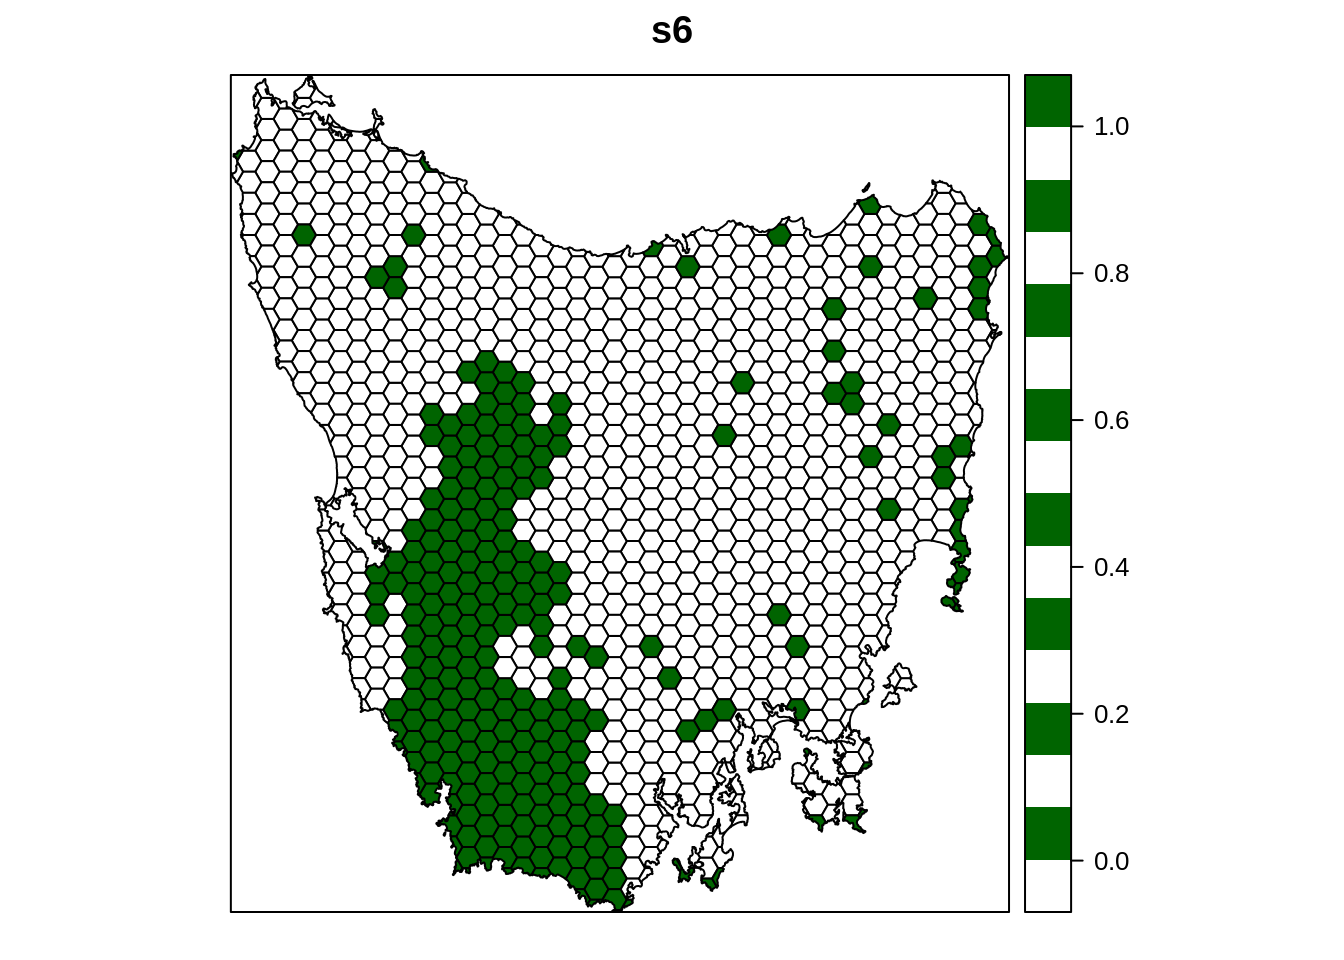
\includegraphics[width=0.65\linewidth]{prioritizr-workshop-manual_files/figure-latex/budget-1} \end{center}

\begin{Shaded}
\begin{Highlighting}[]
\CommentTok{# calculate feature representation}
\NormalTok{r6 <-}\StringTok{ }\KeywordTok{feature_representation}\NormalTok{(p6, s6[, }\StringTok{"solution_1"}\NormalTok{])}

\CommentTok{# calculate number of features with targets met}
\KeywordTok{sum}\NormalTok{(r6}\OperatorTok{$}\NormalTok{relative_held }\OperatorTok{>}\StringTok{ }\FloatTok{0.2}\NormalTok{, }\DataTypeTok{na.rm =} \OtherTok{TRUE}\NormalTok{)}
\end{Highlighting}
\end{Shaded}

\begin{verbatim}
## [1] 25
\end{verbatim}

\begin{Shaded}
\begin{Highlighting}[]
\CommentTok{# find out which features have their targets met when we add weights}
\KeywordTok{print}\NormalTok{(r6}\OperatorTok{$}\NormalTok{feature[r6}\OperatorTok{$}\NormalTok{relative_held }\OperatorTok{>}\StringTok{ }\FloatTok{0.2}\NormalTok{])}
\end{Highlighting}
\end{Shaded}

\begin{verbatim}
##  [1] "vegetation.1"  "vegetation.2"  "vegetation.3"  "vegetation.4" 
##  [5] "vegetation.5"  "vegetation.6"  "vegetation.11" "vegetation.12"
##  [9] "vegetation.14" "vegetation.15" "vegetation.17" "vegetation.25"
## [13] "vegetation.28" "vegetation.29" "vegetation.30" "vegetation.32"
## [17] "vegetation.33" "vegetation.34" "vegetation.35" "vegetation.36"
## [21] "vegetation.37" "vegetation.38" "vegetation.39" "vegetation.40"
## [25] "vegetation.45" NA
\end{verbatim}

We can also add weights to specify that it is more important to meet the
targets for certain features and less important for other features. A
common approach for weighting features is to assign a greater importance
to features with smaller spatial distributions. The rationale behind
this weighting method is that features with smaller spatial
distributions are at greater risk of extinction. So, let's calculate
some weights for our vegetation communities and see how weighting the
features changes our prioritization.

\begin{Shaded}
\begin{Highlighting}[]
\CommentTok{# calculate weights as the log inverse number of grid cells that each vegetation}
\CommentTok{# class occupies, rescaled between 1 and 100}
\NormalTok{wts <-}\StringTok{ }\DecValTok{1} \OperatorTok{/}\StringTok{ }\KeywordTok{cellStats}\NormalTok{(veg_data, }\StringTok{"sum"}\NormalTok{)}
\NormalTok{wts <-}\StringTok{ }\KeywordTok{rescale}\NormalTok{(wts, }\DataTypeTok{to =} \KeywordTok{c}\NormalTok{(}\DecValTok{1}\NormalTok{, }\DecValTok{10}\NormalTok{))}

\CommentTok{# print the name of the feature with smallest weight}
\KeywordTok{names}\NormalTok{(veg_data)[}\KeywordTok{which.min}\NormalTok{(wts)]}
\end{Highlighting}
\end{Shaded}

\begin{verbatim}
## [1] "vegetation.20"
\end{verbatim}

\begin{Shaded}
\begin{Highlighting}[]
\CommentTok{# print the name of the feature with greatest weight}
\KeywordTok{names}\NormalTok{(veg_data)[}\KeywordTok{which.max}\NormalTok{(wts)]}
\end{Highlighting}
\end{Shaded}

\begin{verbatim}
## [1] "vegetation.52"
\end{verbatim}

\begin{Shaded}
\begin{Highlighting}[]
\CommentTok{# plot histogram of weights}
\KeywordTok{hist}\NormalTok{(wts, }\DataTypeTok{main =} \StringTok{"feature weights"}\NormalTok{)}
\end{Highlighting}
\end{Shaded}

\begin{center}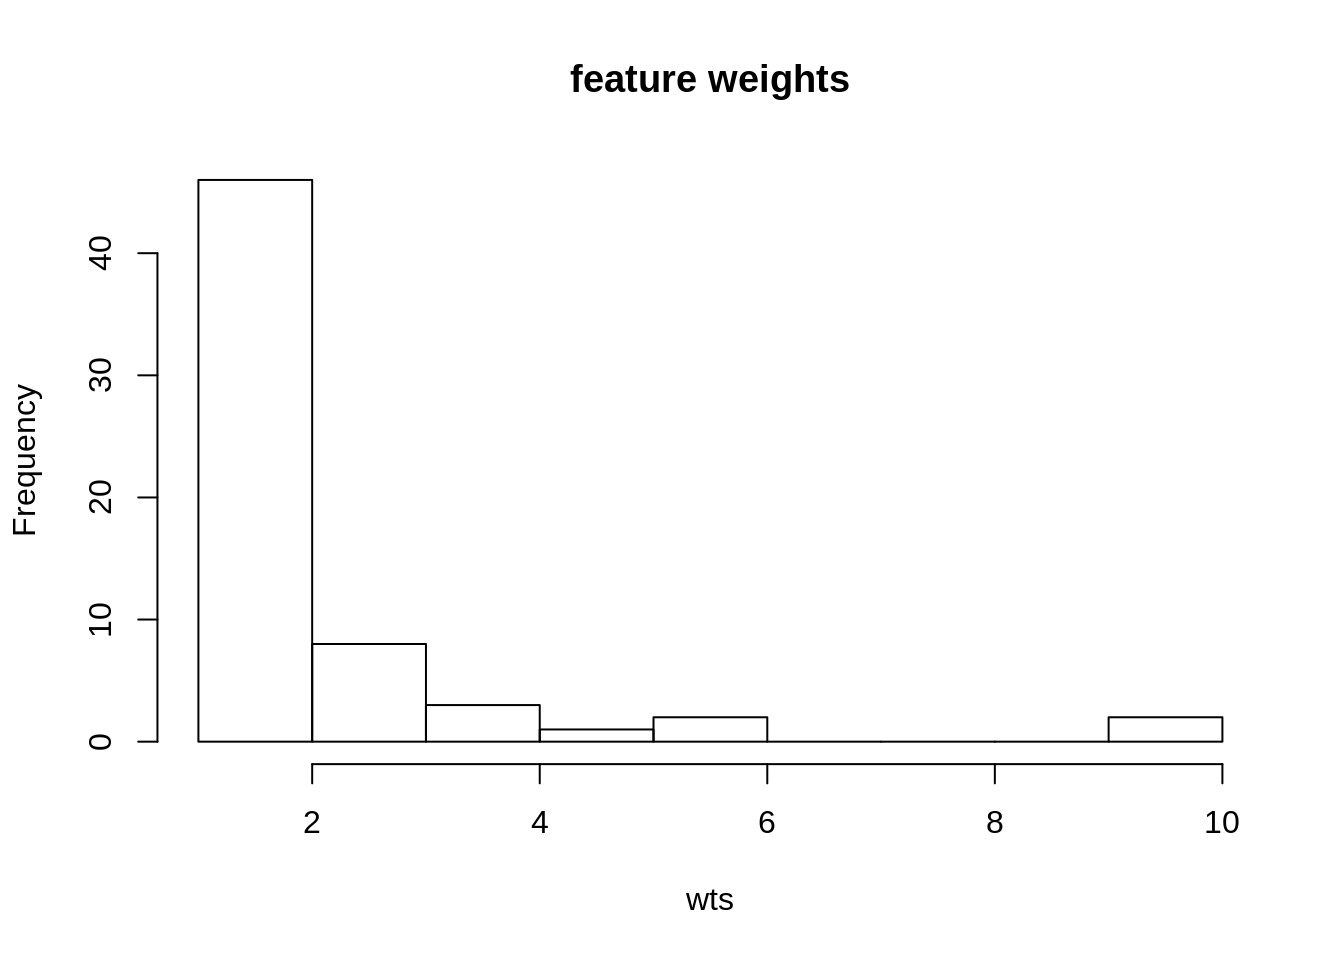
\includegraphics[width=0.65\linewidth]{prioritizr-workshop-manual_files/figure-latex/budget-weights-1} \end{center}

\begin{Shaded}
\begin{Highlighting}[]
\CommentTok{# make prioritization problem with weights}
\NormalTok{p7 <-}\StringTok{ }\KeywordTok{problem}\NormalTok{(pu_data, veg_data, }\DataTypeTok{cost_column =} \StringTok{"cost"}\NormalTok{) }\OperatorTok
\StringTok{      }\KeywordTok{add_max_features_objective}\NormalTok{(budget) }\OperatorTok
\StringTok{      }\KeywordTok{add_relative_targets}\NormalTok{(}\FloatTok{0.2}\NormalTok{) }\OperatorTok
\StringTok{      }\KeywordTok{add_feature_weights}\NormalTok{(wts) }\OperatorTok
\StringTok{      }\KeywordTok{add_locked_in_constraints}\NormalTok{(}\StringTok{"locked_in"}\NormalTok{) }\OperatorTok
\StringTok{      }\KeywordTok{add_locked_out_constraints}\NormalTok{(}\StringTok{"locked_out"}\NormalTok{) }\OperatorTok
\StringTok{      }\KeywordTok{add_binary_decisions}\NormalTok{() }\OperatorTok
\StringTok{      }\KeywordTok{add_lpsymphony_solver}\NormalTok{(}\DataTypeTok{verbose =} \OtherTok{FALSE}\NormalTok{)}

\CommentTok{# print problem}
\KeywordTok{print}\NormalTok{(p7)}
\end{Highlighting}
\end{Shaded}

\begin{verbatim}
## Conservation Problem
##   planning units: SpatialPolygonsDataFrame (1130 units)
##   cost:           min: 0.19249, max: 61.92727
##   features:       vegetation.1, vegetation.2, vegetation.3, ... (62 features)
##   objective:      Maximum representation objective [budget (8575.56009869836)]
##   targets:        Relative targets [targets (min: 0.2, max: 0.2)]
##   decisions:      Binary decision 
##   constraints:    <Locked out planning units [51 locked units]
##                    Locked in planning units [257 locked units]>
##   penalties:      <Feature weights [weights (min: 1, max: 10)]>
##   portfolio:      default
##   solver:         Lpsymphony [first_feasible (0), gap (0.1), time_limit (-1), verbose (0)]
\end{verbatim}

\begin{Shaded}
\begin{Highlighting}[]
\CommentTok{# solve problem}
\NormalTok{s7 <-}\StringTok{ }\KeywordTok{solve}\NormalTok{(p7)}

\CommentTok{# plot solution}
\KeywordTok{spplot}\NormalTok{(s7, }\StringTok{"solution_1"}\NormalTok{, }\DataTypeTok{col.regions =} \KeywordTok{c}\NormalTok{(}\StringTok{"white"}\NormalTok{, }\StringTok{"darkgreen"}\NormalTok{), }\DataTypeTok{main =} \StringTok{"s7"}\NormalTok{)}
\end{Highlighting}
\end{Shaded}

\begin{center}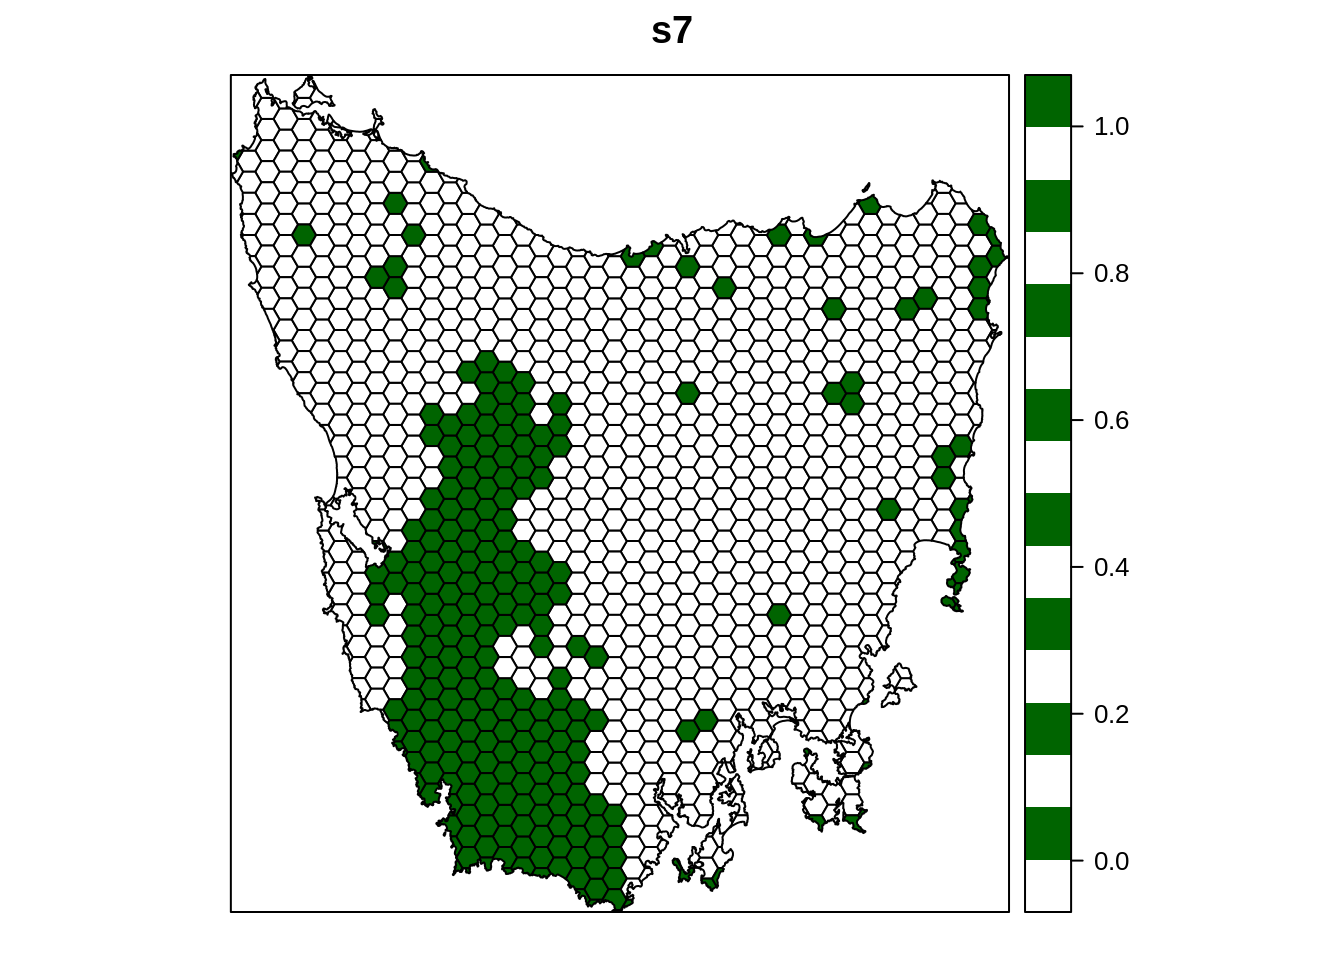
\includegraphics[width=0.65\linewidth]{prioritizr-workshop-manual_files/figure-latex/budget-weights-2} \end{center}

\begin{Shaded}
\begin{Highlighting}[]
\CommentTok{# calculate feature representation}
\NormalTok{r7 <-}\StringTok{ }\KeywordTok{feature_representation}\NormalTok{(p7, s7[, }\StringTok{"solution_1"}\NormalTok{])}

\CommentTok{# calculate number of features with targets met}
\KeywordTok{sum}\NormalTok{(r7}\OperatorTok{$}\NormalTok{relative_held }\OperatorTok{>}\StringTok{ }\FloatTok{0.2}\NormalTok{, }\DataTypeTok{na.rm =} \OtherTok{TRUE}\NormalTok{)}
\end{Highlighting}
\end{Shaded}

\begin{verbatim}
## [1] 25
\end{verbatim}

\begin{Shaded}
\begin{Highlighting}[]
\CommentTok{# find out which features have their targets met when we add weights}
\KeywordTok{print}\NormalTok{(r7}\OperatorTok{$}\NormalTok{feature[r7}\OperatorTok{$}\NormalTok{relative_held }\OperatorTok{>}\StringTok{ }\FloatTok{0.2}\NormalTok{])}
\end{Highlighting}
\end{Shaded}

\begin{verbatim}
##  [1] "vegetation.1"  "vegetation.2"  "vegetation.4"  "vegetation.5" 
##  [5] "vegetation.6"  "vegetation.8"  "vegetation.11" "vegetation.28"
##  [9] "vegetation.29" "vegetation.30" "vegetation.32" "vegetation.33"
## [13] "vegetation.34" "vegetation.35" "vegetation.36" "vegetation.37"
## [17] "vegetation.38" "vegetation.39" "vegetation.40" "vegetation.45"
## [21] "vegetation.49" "vegetation.50" "vegetation.52" "vegetation.53"
## [25] "vegetation.55" NA
\end{verbatim}

\BeginKnitrBlock{rmdquestion}
\begin{enumerate}
\def\labelenumi{\arabic{enumi}.}
\tightlist
\item
  What is the name of the feature with the smallest weight?
\item
  What is the cost of the sixth (\texttt{s6}) and seventh (\texttt{s7})
  solutions?
\item
  Does there seem to be a big difference in which planning units were
  selected in the sixth (\texttt{s6}) and seventh (\texttt{s7})
  solutions?
\item
  Is there a difference between which features are adequately
  represented in the sixth (\texttt{s6}) and seventh (\texttt{s7})
  solutions?
\end{enumerate}
\EndKnitrBlock{rmdquestion}

\section{Solution portfolios}\label{solution-portfolios}

In systematic conservation planning, only rarely do we have data on all
of the stakeholder preferences and biodiversity features that we are
interested in conserving. As a consequence, it is often useful to
generate a portfolio of near optimal solutions to present to decision
makers to guide the reserve selection process. Generally we would want
many solutions in our portfolio (e.g.~1000) to ensure that our portfolio
contains a range of highly different solutions, but here we will
generate a portfolio containing just six near-optimal solutions so the
code doesn't take too long to run. We will also increase the optimality
gap to obtain solutions that are more suboptimal than earlier (the
default gap value is 0.1).

\begin{Shaded}
\begin{Highlighting}[]
\CommentTok{# make problem with a shuffle portfolio}
\NormalTok{p8 <-}\StringTok{ }\KeywordTok{problem}\NormalTok{(pu_data, veg_data, }\DataTypeTok{cost_column =} \StringTok{"cost"}\NormalTok{) }\OperatorTok
\StringTok{      }\KeywordTok{add_max_features_objective}\NormalTok{(budget) }\OperatorTok
\StringTok{      }\KeywordTok{add_relative_targets}\NormalTok{(}\FloatTok{0.2}\NormalTok{) }\OperatorTok
\StringTok{      }\KeywordTok{add_feature_weights}\NormalTok{(wts) }\OperatorTok
\StringTok{      }\KeywordTok{add_binary_decisions}\NormalTok{() }\OperatorTok
\StringTok{      }\KeywordTok{add_shuffle_portfolio}\NormalTok{(}\DataTypeTok{number_solutions =} \DecValTok{6}\NormalTok{,}
                            \DataTypeTok{remove_duplicates =} \OtherTok{FALSE}\NormalTok{) }\OperatorTok
\StringTok{      }\KeywordTok{add_lpsymphony_solver}\NormalTok{(}\DataTypeTok{verbose =} \OtherTok{TRUE}\NormalTok{, }\DataTypeTok{gap =} \DecValTok{10}\NormalTok{)}

\CommentTok{# print problem}
\KeywordTok{print}\NormalTok{(p8)}
\end{Highlighting}
\end{Shaded}

\begin{verbatim}
## Conservation Problem
##   planning units: SpatialPolygonsDataFrame (1130 units)
##   cost:           min: 0.19249, max: 61.92727
##   features:       vegetation.1, vegetation.2, vegetation.3, ... (62 features)
##   objective:      Maximum representation objective [budget (8575.56009869836)]
##   targets:        Relative targets [targets (min: 0.2, max: 0.2)]
##   decisions:      Binary decision 
##   constraints:    <none>
##   penalties:      <Feature weights [weights (min: 1, max: 10)]>
##   portfolio:      Shuffle portfolio [number_solutions (6), remove_duplicates (0), threads (1)]
##   solver:         Lpsymphony [first_feasible (0), gap (10), time_limit (-1), verbose (1)]
\end{verbatim}

\begin{Shaded}
\begin{Highlighting}[]
\CommentTok{# solve problem}
\CommentTok{# note that this will contain six solutions since we added a portfolio}
\NormalTok{s8 <-}\StringTok{ }\KeywordTok{solve}\NormalTok{(p8)}

\CommentTok{# print solution}
\KeywordTok{print}\NormalTok{(s8)}
\end{Highlighting}
\end{Shaded}

\begin{verbatim}
## class       : SpatialPolygonsDataFrame 
## features    : 1130 
## extent      : 1080623, 1399989, -4840595, -4497092  (xmin, xmax, ymin, ymax)
## crs         : +proj=aea +lat_1=-18 +lat_2=-36 +lat_0=0 +lon_0=132 +x_0=0 +y_0=0 +ellps=GRS80 +units=m +no_defs 
## variables   : 12
## names       :   id,              cost, status, locked_in, locked_out, pa_status, solution_1, solution_2, solution_3, solution_4, solution_5, solution_6 
## min values  :    1, 0.192488262910798,      0,         0,          0,         0,          0,          0,          0,          0,          0,          0 
## max values  : 1130,  61.9272727272727,      2,         1,          1,         1,          1,          1,          1,          1,          1,          1
\end{verbatim}

\begin{Shaded}
\begin{Highlighting}[]
\CommentTok{# plot first solution}
\KeywordTok{spplot}\NormalTok{(s8, }\StringTok{"solution_1"}\NormalTok{, }\DataTypeTok{col.regions =} \KeywordTok{c}\NormalTok{(}\StringTok{"white"}\NormalTok{, }\StringTok{"darkgreen"}\NormalTok{),}
       \DataTypeTok{main =} \StringTok{"s8 (solution 1)"}\NormalTok{)}
\end{Highlighting}
\end{Shaded}

\begin{center}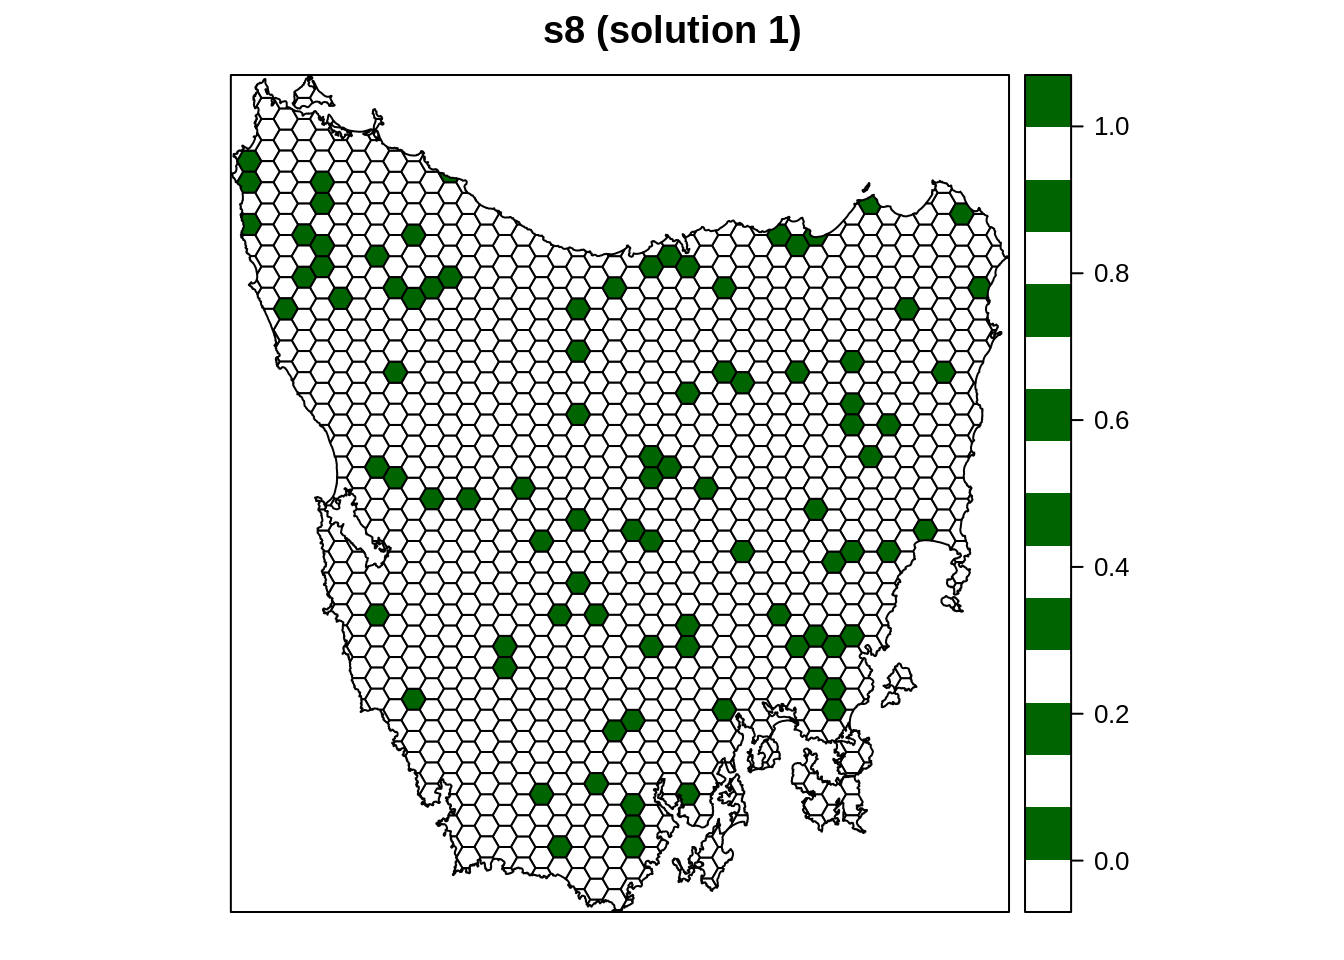
\includegraphics[width=0.65\linewidth]{prioritizr-workshop-manual_files/figure-latex/unnamed-chunk-46-1} \end{center}

\begin{Shaded}
\begin{Highlighting}[]
\CommentTok{# plot all solutions}
\NormalTok{s8_plots <-}\StringTok{ }\KeywordTok{lapply}\NormalTok{(}\KeywordTok{paste0}\NormalTok{(}\StringTok{"solution_"}\NormalTok{, }\KeywordTok{seq_len}\NormalTok{(}\DecValTok{6}\NormalTok{)), }\ControlFlowTok{function}\NormalTok{(x) \{}
  \KeywordTok{spplot}\NormalTok{(s8, x, }\DataTypeTok{main =}\NormalTok{ x, }\DataTypeTok{col.regions =} \KeywordTok{c}\NormalTok{(}\StringTok{"white"}\NormalTok{, }\StringTok{"darkgreen"}\NormalTok{))}
\NormalTok{\})}
\KeywordTok{do.call}\NormalTok{(grid.arrange, }\KeywordTok{append}\NormalTok{(s8_plots, }\KeywordTok{list}\NormalTok{(}\DataTypeTok{ncol =} \DecValTok{3}\NormalTok{)))}
\end{Highlighting}
\end{Shaded}

\begin{center}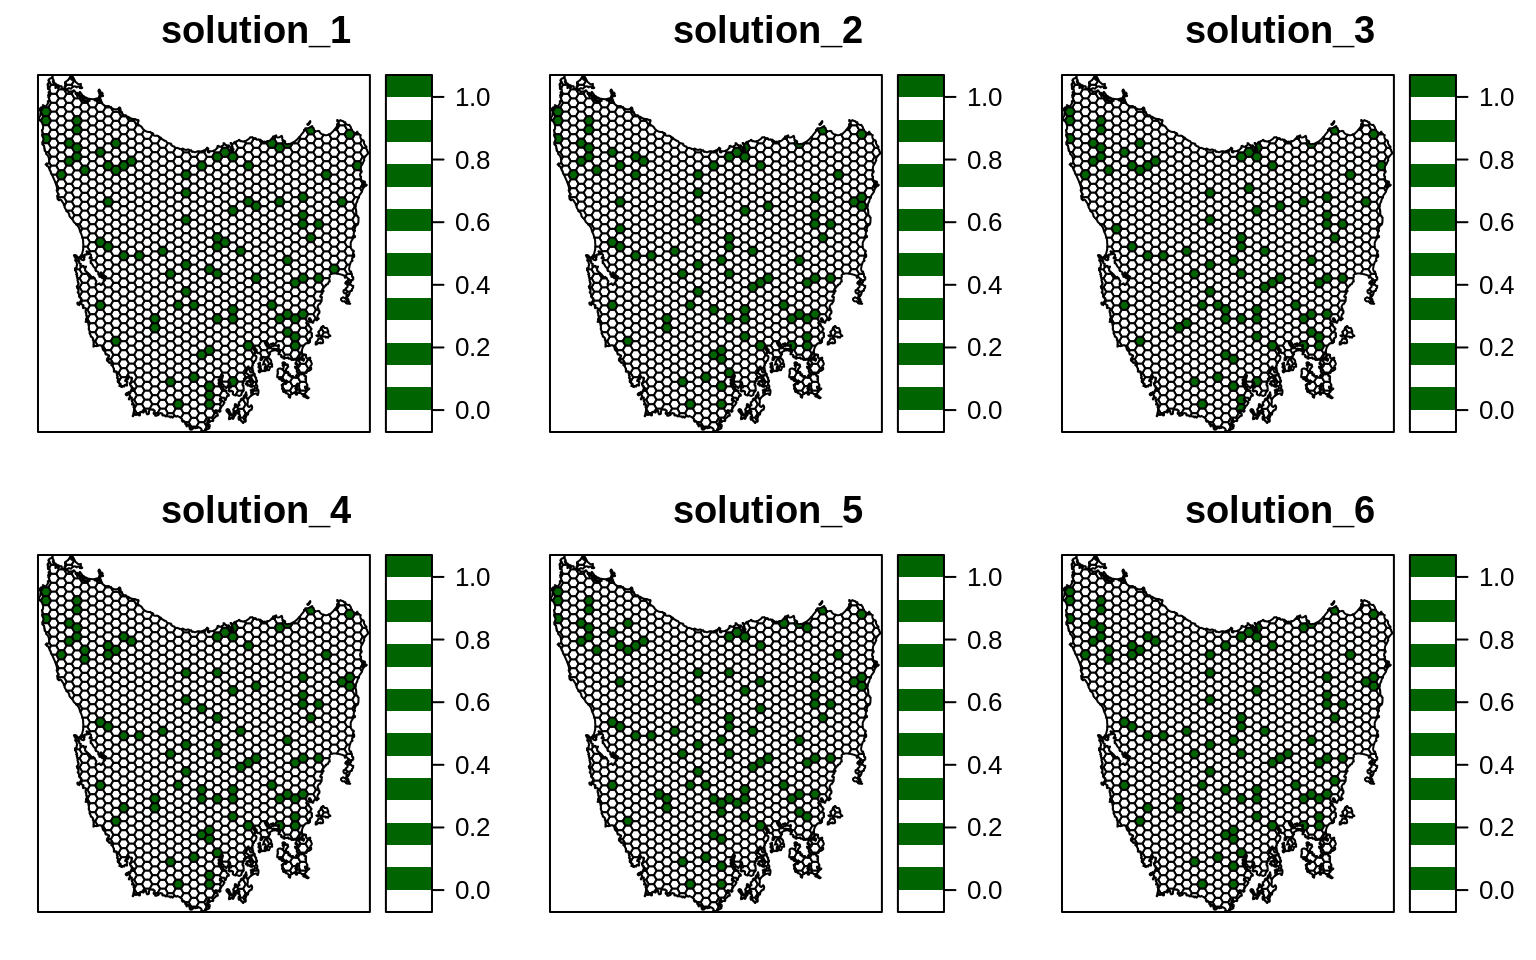
\includegraphics{prioritizr-workshop-manual_files/figure-latex/unnamed-chunk-47-1} \end{center}

\begin{Shaded}
\begin{Highlighting}[]
\CommentTok{# calculate the cost of the first solution}
\KeywordTok{sum}\NormalTok{(s8}\OperatorTok{$}\NormalTok{solution_}\DecValTok{1} \OperatorTok{*}\StringTok{ }\NormalTok{s8}\OperatorTok{$}\NormalTok{cost)}
\end{Highlighting}
\end{Shaded}

\begin{verbatim}
## [1] 2194.232
\end{verbatim}

\begin{Shaded}
\begin{Highlighting}[]
\CommentTok{# calculate the cost of the second solution}
\KeywordTok{sum}\NormalTok{(s8}\OperatorTok{$}\NormalTok{solution_}\DecValTok{2} \OperatorTok{*}\StringTok{ }\NormalTok{s8}\OperatorTok{$}\NormalTok{cost)}
\end{Highlighting}
\end{Shaded}

\begin{verbatim}
## [1] 2148.593
\end{verbatim}

\begin{Shaded}
\begin{Highlighting}[]
\CommentTok{# calculate the proportion of planning units with the same solution values}
\CommentTok{# in the first and second solutions}
\KeywordTok{mean}\NormalTok{(s8}\OperatorTok{$}\NormalTok{solution_}\DecValTok{1} \OperatorTok{==}\StringTok{ }\NormalTok{s8}\OperatorTok{$}\NormalTok{solution_}\DecValTok{2}\NormalTok{)}
\end{Highlighting}
\end{Shaded}

\begin{verbatim}
## [1] 0.979646
\end{verbatim}

\BeginKnitrBlock{rmdquestion}
\begin{enumerate}
\def\labelenumi{\arabic{enumi}.}
\tightlist
\item
  What is the cost of each of the six solutions in portfolio? Are their
  costs very different?
\item
  Are the solutions in the portfolio very different?
\item
  What could we do to obtain a portfolio with more different solutions?
\end{enumerate}
\EndKnitrBlock{rmdquestion}

\chapter{Answers}\label{answers}

This chapter contains the answers to the questions presented in the
earlier chapters. The answers are provided here so you can check if your
answers are correct.

\section{Data}\label{data}

\subsection{Planning unit data}\label{planning-unit-data-1}

\BeginKnitrBlock{rmdanswer}
\begin{enumerate}
\def\labelenumi{\arabic{enumi}.}
\tightlist
\item
  \texttt{nrow(pu\_data)}
\item
  \texttt{max(pu\_data\$cost)}
\item
  \texttt{sum(pu\_data\$locked\_in)}
\item
  \texttt{mean(pu\_data\$locked\_in)}
\item
  \texttt{sum(pu\_data\$locked\_out)}
\item
  \texttt{mean(pu\_data\$locked\_out)}
\item
  \texttt{assert\_that(min(c(pu\_data\$locked\_in,\ pu\_data\$locked\_out))\ ==\ 0)}
  \newline

  \texttt{assert\_that(max(c(pu\_data\$locked\_in,\ pu\_data\$locked\_out))\ ==\ 1)}
\item
  \texttt{all(is.finite(pu\_data\$cost))}
\item
  \texttt{assert\_that(sum(duplicated(pu\_data\$id))\ ==\ 0)}
\item
  Yes, the eastern side of Tasmania is generally much cheaper than the
  western side.
\item
  Yes, most planning units covered by protected areas are located in the
  south-western side of Tasmania.
\end{enumerate}
\EndKnitrBlock{rmdanswer}

\subsection{Vegetation data}\label{vegetation-data-1}

\BeginKnitrBlock{rmdanswer}
\begin{enumerate}
\def\labelenumi{\arabic{enumi}.}
\tightlist
\item
  Central-north Tasmania
\item
  \texttt{cellStats(veg\_data{[}{[}12{]}{]},\ "mean")}
\item
  \texttt{names(veg\_data){[}which.max(cellStats(veg\_data,\ "sum")){]}}
\end{enumerate}
\EndKnitrBlock{rmdanswer}

\section{Gap analysis}\label{gap-analysis}

\subsection{Feature abundance}\label{feature-abundance-1}

\BeginKnitrBlock{rmdanswer}
\begin{enumerate}
\def\labelenumi{\arabic{enumi}.}
\tightlist
\item
  \texttt{median(abundance\_data\$absolute\_abundance\_km2)}
\item
  \texttt{min(abundance\_data\$absolute\_abundance\_km2)}
\item
  \texttt{abundance\_data\$feature{[}which.min(abundance\_data\$absolute\_abundance\_km2){]}}
\item
  \texttt{sum(abundance\_data\$absolute\_abundance\_km2)}
\item
  \texttt{sum(abundance\_data\$absolute\_abundance\_km2\ \textgreater{}\ set\_units(100,\ km\^{}2))}
\end{enumerate}
\EndKnitrBlock{rmdanswer}

\subsection{Feature representation by protected
areas}\label{feature-representation-by-protected-areas-1}

\BeginKnitrBlock{rmdanswer}
\begin{enumerate}
\def\labelenumi{\arabic{enumi}.}
\tightlist
\item
  \texttt{mean(repr\_data\$relative\_held,\ na.rm\ =\ TRUE)}
\item
  \texttt{mean(repr\_data\$absolute\_held\_km2,\ na.rm\ =\ TRUE)}
\item
  \texttt{repr\_data\$feature{[}which.max(repr\_data\$relative\_held){]}}
\item
  \texttt{repr\_data\$feature{[}which.max(repr\_data\$absolute\_held){]}}
\item
  No, just because a vegetation class is widespread does not necessarily
  mean that it has the greatest overlap with protected areas. In fact,
  due to biases in the establishment of protected areas this can often
  be the case.
\item
  Yes, the largest protected areas tend to have the great representation
  (broadly speaking). \newline
  See
  \texttt{plot(x\ =\ abundance\_data\$absolute\_abundance,\ y\ =\ repr\_data\$relative\_held)}
\item
  \texttt{sum(repr\_data\$absolute\_held\ \textless{}\ 1e-10)} (floating
  point errors)
\item
  \texttt{sum(repr\_data\$relative\_held\ \textgreater{}\ 0.1)}
\item
  \texttt{sum(repr\_data\$relative\_held\ \textgreater{}\ 0.2)}
\end{enumerate}
\EndKnitrBlock{rmdanswer}

\section{Spatial prioritizations}\label{spatial-prioritizations}

\subsection{Starting out simple}\label{starting-out-simple-1}

\BeginKnitrBlock{rmdanswer}
\begin{enumerate}
\def\labelenumi{\arabic{enumi}.}
\tightlist
\item
  \texttt{sum(s1\$solution\_1)} \newline
   \texttt{mean(s1\$solution\_1)}
\item
  Yes, the planning units are generally spread out across most of the
  study area and they are not biased towards specific areas.
\item
  \texttt{all(feature\_representation(p1,\ s1{[},\ "solution\_1"{]})\$relative\_held\ \textgreater{}=\ 0.2)}
\item
  This prioritization (i) does not account for existing protected areas,
  (ii) does not account for the spatial fragmentation of priority areas,
  or (iii) is not likely conserve enough habitat for each vegetation
  type (i.e.~5\% is pretty small).
\end{enumerate}
\EndKnitrBlock{rmdanswer}

\subsection{Adding complexity}\label{adding-complexity-1}

\BeginKnitrBlock{rmdanswer}
\begin{enumerate}
\def\labelenumi{\arabic{enumi}.}
\tightlist
\item
  \texttt{sum(s2\$cost\ *\ s2\$solution\_1)} \newline
   \texttt{sum(s3\$cost\ *\ s3\$solution\_1)} \newline
   \texttt{sum(s4\$cost\ *\ s4\$solution\_1)}
\item
  \texttt{sum(s2\$solution\_1)} \newline
   \texttt{sum(s3\$solution\_1)} \newline
   \texttt{sum(s4\$solution\_1)}
\item
  No, just because a solution a solution has more planning units does
  not mean that it will cost less.
\item
  This is because the planning units covered by existing protected areas
  have a non-zero cost and locking in these planning units introduces
  inefficiencies into the solution. This is very common in real-world
  conservation prioritizations because existing protected areas are
  often in places that do little to benefit biodiversity \citep{r3}.
\item
  This is because some of the planning units that are highly degraded --
  based on just the planning unit costs and vegetation data -- provide
  cost-efficient opportunities for meeting the targets and excluding
  them from the reserve selection process means that other more costly
  planning units are needed to meet the targets.
\item
  \texttt{sum(s4\$cost\ *\ s4\$solution\_1)\ -\ sum(s4\$cost\ *\ s4\$locked\_in)}
\item
  We get an error message stating the the problem is infeasible because
  there is no valid solution---even if we selected all the planning
  units the study area we would still not meet the targets.
\end{enumerate}
\EndKnitrBlock{rmdanswer}

\subsection{Penalizing fragmentation}\label{penalizing-fragmentation-1}

\BeginKnitrBlock{rmdanswer}
\begin{enumerate}
\def\labelenumi{\arabic{enumi}.}
\tightlist
\item
  The cost of the fourth solution is
  \texttt{sum(s4\$solution\_1\ *\ s4\$cost)} and the cost of the fifth
  solution is \texttt{sum(s5\$solution\_1\ *\ s5\$cost)}. The fifth
  solution (\texttt{s5}) costs more than the fourth solution
  (\texttt{s4}) because we have added penalties to the conservation
  planning problem to indicate that we are willing to accept a slightly
  more costly solution if it means that we can reduce fragmentation.
\item
  The solution is now nearly identical to the fourth solution
  (\texttt{s4}) and so has nearly the same cost. This penalty value is
  too low and is not useful because it does not reduce the fragmentation
  in our solution.
\item
  The solution now contains a lot of extra planning units that are not
  needed to meet our targets. In fact, nearly every planning unit in the
  study is now selected. This penalty value is too high and is not
  useful.
\end{enumerate}
\EndKnitrBlock{rmdanswer}

\subsection{Budget limited
prioritizations}\label{budget-limited-prioritizations-1}

\BeginKnitrBlock{rmdanswer}
\begin{enumerate}
\def\labelenumi{\arabic{enumi}.}
\tightlist
\item
  \texttt{names(veg\_data){[}which.min(wts){]}}
\item
  \texttt{sum(s6\$cost\ *\ s6\$solution\_1)} \newline
   \texttt{sum(s7\$cost\ *\ s7\$solution\_1)}
\item
  No, the sixth (\texttt{s6}) and seventh (\texttt{s7}) solutions both
  share many of the same selected planning units and there does not
  appear to be specific difference in the spatial location of the
  planning units which they do not share.
\item
  Yes. Although both of these solutions are meeting the targets for
  \texttt{r6\$feature{[}r6\$relative\_held\ \textgreater{}\ 0.2\ \&\ r7\$relative\_held\ \textgreater{}\ 0.2{]}}
  vegetation communities, the sixth (\texttt{s6}) is also adequately
  representing
  \texttt{r6\$feature{[}r6\$relative\_held\ \textgreater{}\ 0.2\ \&\ !r7\$relative\_held\ \textgreater{}\ 0.2{]}}
  additional community and the seventh (\texttt{s7}) solution is
  adequately representing
  \texttt{r6\$feature{[}!r6\$relative\_held\ \textgreater{}\ 0.2\ \&\ r7\$relative\_held\ \textgreater{}\ 0.2{]}}
  different additional community.
\end{enumerate}
\EndKnitrBlock{rmdanswer}

\subsection{Solution portfolios}\label{solution-portfolios-1}

\BeginKnitrBlock{rmdanswer}
\begin{enumerate}
\def\labelenumi{\arabic{enumi}.}
\tightlist
\item
  No the cost are very similar. \newline
   \texttt{sum(s8\$solution\_1\ *\ s8\$cost)} \newline
   \texttt{sum(s8\$solution\_2\ *\ s8\$cost)} \newline
   \texttt{sum(s8\$solution\_3\ *\ s8\$cost)} \newline
   \texttt{sum(s8\$solution\_4\ *\ s8\$cost)} \newline
   \texttt{sum(s8\$solution\_5\ *\ s8\$cost)} \newline
   \texttt{sum(s8\$solution\_6\ *\ s8\$cost)}
\item
  No the status of the planning units are very similar in the all of the
  solutions in the portfolio. \newline
  \texttt{mean((s8\$solution\_1\ ==\ s8\$solution\_2)\ \&\ (s8\$solution\_1\ ==\ s8\$solution\_3)\ \&\ (s8\$solution\_1\ ==\ s8\$solution\_4)\ \&\ (s8\$solution\_1\ ==\ s8\$solution\_5)\ \&\ (s8\$solution\_1\ ==\ s8\$solution\_6))}
\item
  We should increase the number of the solutions in the portfolio.
\end{enumerate}
\EndKnitrBlock{rmdanswer}

\chapter{Acknowledgements}\label{acknowledgements}

Many thanks to \href{https://icons8.com}{Icons8} for providing the icons
used in this manual and to Yihui Xie for developing the
\href{http://bookdown.org}{bookdown R package} that underpins this
manual.

\chapter{Session information}\label{session-information}

\begin{Shaded}
\begin{Highlighting}[]
\CommentTok{# print session information}
\KeywordTok{sessionInfo}\NormalTok{()}
\end{Highlighting}
\end{Shaded}

\begin{verbatim}
## R version 3.6.1 (2017-01-27)
## Platform: x86_64-pc-linux-gnu (64-bit)
## Running under: Ubuntu 16.04.6 LTS
## 
## Matrix products: default
## BLAS:   /home/travis/R-bin/lib/R/lib/libRblas.so
## LAPACK: /home/travis/R-bin/lib/R/lib/libRlapack.so
## 
## locale:
##  [1] LC_CTYPE=en_US.UTF-8       LC_NUMERIC=C              
##  [3] LC_TIME=en_US.UTF-8        LC_COLLATE=en_US.UTF-8    
##  [5] LC_MONETARY=en_US.UTF-8    LC_MESSAGES=en_US.UTF-8   
##  [7] LC_PAPER=en_US.UTF-8       LC_NAME=C                 
##  [9] LC_ADDRESS=C               LC_TELEPHONE=C            
## [11] LC_MEASUREMENT=en_US.UTF-8 LC_IDENTIFICATION=C       
## 
## attached base packages:
## [1] stats     graphics  grDevices utils     datasets  methods   base     
## 
## other attached packages:
##  [1] gridExtra_2.3    assertthat_0.2.1 scales_1.0.0     units_0.6-4     
##  [5] mapview_2.7.0    rgeos_0.5-2      rgdal_1.4-6      prioritizr_4.1.4
##  [9] proto_1.0.0      raster_3.0-7     sp_1.3-1         forcats_0.4.0   
## [13] stringr_1.4.0    dplyr_0.8.3      purrr_0.3.2      readr_1.3.1     
## [17] tidyr_1.0.0      tibble_2.1.3     ggplot2_3.2.1    tidyverse_1.2.1 
## 
## loaded via a namespace (and not attached):
##  [1] nlme_3.1-140       sf_0.8-0           satellite_1.0.1   
##  [4] lubridate_1.7.4    webshot_0.5.1      httr_1.4.1        
##  [7] tools_3.6.1        backports_1.1.5    utf8_1.1.4        
## [10] R6_2.4.0           KernSmooth_2.23-15 DBI_1.0.0         
## [13] lazyeval_0.2.2     colorspace_1.4-1   withr_2.1.2       
## [16] tidyselect_0.2.5   leaflet_2.0.2      compiler_3.6.1    
## [19] cli_1.1.0          rvest_0.3.4        xml2_1.2.2        
## [22] bookdown_0.14.1    classInt_0.4-1     digest_0.6.21     
## [25] rmarkdown_1.16     base64enc_0.1-3    pkgconfig_2.0.3   
## [28] htmltools_0.4.0    lpsymphony_1.12.0  htmlwidgets_1.5   
## [31] rlang_0.4.0        readxl_1.3.1       rstudioapi_0.10   
## [34] shiny_1.3.2        generics_0.0.2     jsonlite_1.6      
## [37] crosstalk_1.0.0    magrittr_1.5       Matrix_1.2-17     
## [40] Rcpp_1.0.2         munsell_0.5.0      fansi_0.4.0       
## [43] lifecycle_0.1.0    stringi_1.4.3      yaml_2.2.0        
## [46] plyr_1.8.4         grid_3.6.1         parallel_3.6.1    
## [49] promises_1.1.0     crayon_1.3.4       lattice_0.20-38   
## [52] haven_2.1.1        hms_0.5.1          zeallot_0.1.0     
## [55] knitr_1.25         pillar_1.4.2       uuid_0.1-2        
## [58] velox_0.2.0        codetools_0.2-16   stats4_3.6.1      
## [61] glue_1.3.1         evaluate_0.14      modelr_0.1.5      
## [64] png_0.1-7          vctrs_0.2.0        httpuv_1.5.2      
## [67] cellranger_1.1.0   gtable_0.3.0       xfun_0.10         
## [70] mime_0.7           xtable_1.8-4       broom_0.5.2       
## [73] e1071_1.7-2        later_1.0.0        class_7.3-15      
## [76] viridisLite_0.3.0
\end{verbatim}

\bibliography{references.bib}


\end{document}
